\documentclass[fleqn]{article}

\usepackage{arxiv}

\usepackage{mypackages}
\bibliography{~/Desktop/icloud/MyRefGlobal}
\usepackage{mycommands}

\usepackage[utf8]{inputenc} % allow utf-8 input
\usepackage[T1]{fontenc}    % use 8-bit T1 fonts
\usepackage{hyperref}       % hyperlinks
\usepackage{url}            % simple URL typesetting
\usepackage{booktabs}       % professional-quality tables
\usepackage{amsfonts}       % blackboard math symbols
\usepackage{nicefrac}       % compact symbols for 1/2, etc.
\usepackage{microtype}      % microtypography
\usepackage{cleveref}       % smart cross-referencing
\usepackage{lipsum}         % Can be removed after putting your text content
\usepackage{graphicx}
\usepackage{doi}

\usepackage{float}

\title{Language models as probabilistic cognitive models}

\date{}

\newif\ifuniqueAffiliation
% Uncomment to use multiple affiliations variant of author block
\uniqueAffiliationtrue

\ifuniqueAffiliation % Standard variant of author block
  \author{ Michael Franke\thanks{Corresponding author.} \\
	Department of Linguistics\\
	University of Tübingen\\
	\texttt{mchfranke@uni-tuebingen.de} \\
	%% examples of more authors
	\And
	Polina Tsvilodub \\
	Department of Linguistics\\
	University of Tübingen\\
	\texttt{polina.tsvilodub@gmail.com} \\
	\And
	Fausto Carcassi \\
	ILLC\\
	University of Amsterdam\\
	\texttt{fausto.carcassi@gmail.com} \\
}
\else
% Multiple affiliations variant of author block
\usepackage{authblk}
\renewcommand\Authfont{\bfseries}
\setlength{\affilsep}{0em}
% box is needed for correct spacing with authblk
% \newbox{\orcid}\sbox{\orcid}{\includegraphics[scale=0.06]{orcid.pdf}}
\author{Michael Franke, Polina Tsvilodub, Fausto Carcassi}
\affil{Department of Linguistics\\University of Tübingen\\
\texttt{[michael.franke|polina.tsvilodub|fausto.carcassi]@uni-tuebingen.de}}
\fi

% running right header
\renewcommand{\headeright}{}
% small title under big title
\renewcommand{\undertitle}{}
\renewcommand{\shorttitle}{Statistical modeling with LLM predictors}

%%% Add PDF metadata to help others organize their library
%%% Once the PDF is generated, you can check the metadata with
%%% $ pdfinfo template.pdf
\hypersetup{
pdftitle={Statistical modeling with LLM predictors},
pdfsubject={},
pdfauthor={Michael Franke, Polina Tsvilodub, Fausto Carcassi},
pdfkeywords={statistical models, language use, large language models, Bayesian data analysis, reference games},
}

\begin{document}
\maketitle

\begin{abstract}
  State of the art large language models (LLMs) have shown impressive performance on a variety of benchmark tasks and are increasingly used as components in larger applications, where LLM-based predictions serve as proxies for human judgements.
  This raises questions about the human-likeness of LLM-derived information and whether LLMs, if they deliver human-like behavior, could possibly be considered explanatory models of (aspects of) human cognition or language use.
  To shed more light on these issues, we here investigate the human-likeness of LLMs' predictions for multiple-choice decision tasks from the perspective of probabilistic cognitive modeling.
  We identify core differences, in terms of conceptual interpretation and usual practical evaluation, between LLMs and probabilistic cognitive models (PCMs).
  Concretely, we argue that LLMs are, first and foremost, predictors of item-level data, whereas PCMs primarily make predictions at a more abstract level (the condition-level), and that this is a sense in which LLMs may be said to be not explanatory.
  Using human data from a multiple-choice experiment on pragmatic language use, we find that LLMs fail to capture the variance in the human data at the item-level.
  We suggest different ways of deriving full distributional predictions from LLMs for condition-level data, thus building PCM-like predictions from LLM-derived information, and find that some, but not all ways of obtaining condition-level predictions yield adequate fits to our data.
  These results suggests that assessment of LLM performance depends strongly on seemingly subtle choices in methodology, and that LLMs are at best predictors of human behavior at an aggregate level, for which they are, however, not designed to make predictions in the first place.
\end{abstract}


% keywords can be removed
% \keywords{First keyword \and Second keyword \and More}

%%%%%%%%%%%%%%%%%%%%%%%%%%%%%%%%%%%%%%%%%%%%%%%%%%
\section{Introduction}
\label{sec:introduction}
%%%%%%%%%%%%%%%%%%%%%%%%%%%%%%%%%%%%%%%%%%%%%%%%%%

The invention of deep neural transformer architectures \citep{VaswaniShazeer2017:Attention-is-Al} has enabled a new generation of powerful large language models  \citep{DevlinChang2019:BERT:-Pre-train,ChungHou2022:Scaling-Instruc,OpenAI2023:GPT-4-Technical,TouvronLavril2023:LLaMA:-Open-and}.
State-of-the-art LLMs excel on many benchmark data sets \citep[e.g.,][]{srivastava2023-BIGbench,PerezRinger2023:Discovering-Lan}, and so promise to serve as foundation models for a vast and diverse set of applications \citep{BommasaniHudson2021:On-the-opportun}.
% especially when augmented with supervised fine-tuning  \citep{ChungHou2022:Scaling-Instruc} and reinforcement learning from human \citep{StiennonOuyang2022:Learning-to-sum} or other \citep{BaiKadavath2022:Constitutional-} feedback.
Recent works increasingly go beyond using LLMs based on single-run input-output behavior, and instead utilize LLMs as a part of a larger computational process.
Examples include sophisticated prompting strategies \citep[e.g.,][]{LiuLiu2022:Generated-Knowl}, or structured reasoning models \citep[e.g.,][]{CreswellShanahan2022:Selection-Infer,GaoMadaan2023:PAL:-Program-ai,ParanjapeLundberg2023:ART:-Automatic-}.
Information from LLMs is also used  to rank or numerically score options in open-ended applications, e.g., to mimic human judgements of relevance or interestingness \citep[e.g.,][]{ParkOBrien2023:Generative-Agen,ZhangLehman2023:OMNI:-Open-ende}.
Other work, uses LLMs as part of bigger programs to build towards something more akin to explanatory cognitive models \citep[e.g.,][]{WongGrand2023:From-Word-Model}.

For all of these applications, it is crucial to understand what LLMs can or cannot reliably do.
The prevalent approach towards characterizing the capabilities of LLMs relies on benchmark testing, which usually consists in assessing the accuracy of LLM predictions in tasks where a designated ``target answer'' exists, averaged over many instances of this task.
Benchmark-driven assessments are very useful for engineering purposes, e.g., to systematically study of the effects of scale \citep[e.g.,][]{srivastava2023-BIGbench}, but is also used to ask to what extent LLM performance is ``human-like.''
In more psychologically oriented work, LLM performance is therefore compared to human choice behavior in psychological experiments and investigates whether LLMs predict patterns of human answer behavior  \citep[e.g.,][]{BinzSchulz2023:Using-cognitive,Hagendorff2023:Machine-Psychol,ShiffrinMitchell2023:Probing-the-psy}.
The main focus is often to compare qualitative patterns in LLM predictions and human data, but there is also work investigating whether LLMs can make adequate \emph{quantitative predictions}.
For example, work at the interface between NLP and computational psycholinguistics \citep{MarvinLinzen2018:Targeted-Syntac,HuGauthier2020:A-Systematic-As} has evolved into investigations of whether quantitative predictions by LLMs match quantitative aspects in human experimental data, such as reading times \citep{WilcoxVani2021:A-Targeted-Asse} or the amplitude of the N400 component of event-related-potentials in EEG measurements \citep{LindborgRabovsky2021:Meaning-in-brai}.
The work presented in this paper seeks to extend the investigation of the human-likeness of LLMs by looking at empirical data from human multiple-choice behavior and comparing an established, theoretically motivated probabilistic cognitive model, which is commonly use to predict or explain this kind of data, to structurally similar quantitative predictions derived from LLMs.
In short, while a lot of previous work has used targeted assessment of LLM capabilities from the point of view of the experimental psychologist, we here adopt the more specific perspective of the cognitive modeller.

For the purposes of this investigation, a probabilistic cognitive model (PCM) is characterized by providing a parameterized likelihood function $P_{M}(D_{C} \mid \theta, C)$, which assigns a probability to each possible data observation $D_{C}$ for any experimental condition $C$ and parameter values $\theta$ \citep[e.g.,][]{LewandowskyFarrell2011:Computational-M,LeeWagenmakers2013:Bayesian-Cognit}.
% Usually, conditions $C$ provide a categorization of different tasks which is meaningful against the theoretical background of experimental investigation, and parameters $\theta$ modulate the predicted likelihood of the data in human interpretable ways (see Section~\ref{motivation} for more detail).
There are non-trivial, insightful differences between LLMs and PCMs, both at the conceptual level and in terms of common practices in evaluation, which we will explore in this paper in order to contribute to a better delineation of the potential and limitations of LLMs.
For one, the ``primitive predictions'' that LLMs provide are not at the level of a condition $C$, but at a lower item-based level.
% In this sense, LLMs could be said to be less explanatory than PCMs by their very nature (see Section~\ref{motivation}).
For another, LLMs are often just assessed based on their ability to identify a target answer, not to predict the full distribution observed in the data.
% Nevertheless, distributional predictions for condition-level data can in principle be derived from LLMs, but there are many ways of doing so, yet with little consensus of how to do so.

This paper introduces and systematically compares different ways of carving numerical information obtained from an LLM into a structure similar to a parameterized PCM and addresses the empirical question of whether such an ``LLM-based PCM'' adequately captures the distribution of human forced-choice data at different levels of aggregation.
To obtain data for this investigation, we subjected human participants and an LLM (a version of OpenAI's GPT-3.5; see Section~\ref{sec:item-level-pred}) to the same forced-choice task, a simple reference game \citep{FrankGoodman2012:Predicting-Prag}.
We introduce different ways of defining condition-level, distributional predictions based on LLM-provided numerical measures.
We use standard tools of Bayesian data analysis \citep{GelmanCarlin2014:Bayesian-Data-A} to train, test and compare these ``LLM-based PCMs'' against each other, and against an established, theoretically informed PCM, namely the Rational Speech Act (RSA) model \citep{FrankGoodman2012:Predicting-Prag}.
This is quite different, and arguably more stringent and insightful, than the standard practice of evaluating LLMs based on accuracy scores.
We find that variability predicted by the LLM at the item-level is not borne out by the human data, and that some but not all ways of constructing condition-level predictions are equally good.
These results suggest that it is not impossible to build predictive models for condition-level data, similar to PCMs, on top of LLM-supplied information, but that seemingly subtle details in the derivation of likelihoods matter.
The conceptual comparison of LLMs and PCMs also clearly identifies a sense in which the latter are explanatory, while the former are not.

The paper is structured as follows.
Section~\ref{motivation} motivates the investigation in this paper by highlighting relevant differences in the way  LLMs and PCMs make predictions about data from forced-choice tasks.
Section~\ref{experiment-reference-games} looks at human data from a simple but non-trivial forced-choice experiment, namely a text-based reference game, for which Section~\ref{sec:model-pred-from} introduces a commonly used, theoretically-motivate PCM, namely the Rational Speech Act (RSA) model \citep{FrankGoodman2012:Predicting-Prag}.
Section~\ref{sec:item-level-pred} investigates whether LLM-derived item-level predictions adequately capture the human data at the item-level.
Section~\ref{llm-predictions-for-reference-games} then discusses different ways of deriving probabilistic predictions from LLMs at the condition-level and compares them against the human data and each other.

%%%%%%%%%%%%%%%%%%%%%%%%%%%%%%%%%%%%%%%%%%%%%%%%%%
\section{Predictions for multiple-choice tasks from PCMs and LLMs}
\label{motivation}
%%%%%%%%%%%%%%%%%%%%%%%%%%%%%%%%%%%%%%%%%%%%%%%%%%

This section argues that a major conceptual difference between LLMs and PCMs is that they predict data at different levels of abstraction: the item-level and the condition-level, as introduced below.
Another important difference is that PCMs are usually evaluated on a non-degenerate likelihood function, whereas common practice in LLM-evaluation is to use a winner-takes-all strategy.
Problems with this latter strategy are highlighted and alternative ways of defining item- and condition-level predictions from LLMs are introduced for subsequent empirical testing.

\paragraph{Item- and condition-level data.}
Psychological research into the workings of the human mind aims to find generalizable patterns in the way information is processed within or across different domains of cognition.
Experimental work therefore often compares human performance in different \emph{experimental conditions}, which reflect the general factors that are hypothesized to influence behavior.
Yet a single experimental condition is often instantiated with different \emph{experimental items}, which are not under scrutiny for any systematic, predictable effect on the observed measurements.
For example, classical research on human memory \citep{AtkinsonShiffrin1968:Human-memory:-A} investigated the effect of rehearsal on memory consolidation.
Relevant experiments compare recall with and without rehearsal (experimental conditions), while using different items (words, numbers, etc., to be memorized) in each instantiation of the same memory task.
Likewise, when studying how hearing a color word can facilitate a same-or-different judgement of color swatches \citep{Rosch1975:The-Nature-of-M}, the main experimental manipulation concerns the typicality of shown color swatches, while the variability between different color words like ``blue'' or ``green'', is less important to this research question and so treated as \emph{item-level variation}.
Consequently, a typical psychological experiment is mainly interested in assessing behavior at the level of the experimental condition, because that is where the distinctions relevant to the research question reside.
Nevertheless, each experimental condition can be, and often is, instantiated with different items, variation among which is deemed less relevant to the research question at hand.

\paragraph{Probabilistic cognitive models.}
Data from human participants for experiments of this kind usually shows some variability between items, and also variability between participants.
This variability is commonly incorporated in statistical analyses as random stochastic variation, e.g., by using hierarchical (regression) models \citep{Jaeger2008:Categorical-dat,barr2013,SorensenHohensteinb2016:Bayesian-linear}.
Still, the focus of interest usually remains at the condition-level effects, because it is this more abstract level of behavioral aggregation that is relevant for generalizable theory building.
Similarly, when analyzing or explaining data from psychological experiments with a probabilistic cognitive model (PCM), the PCM will naturally be set-up to predict data at the level of the relevant experimental manipulation, i.e., at the condition-level.
Even though item-level (and individual-level) variation can, and sometimes should, be incorporated into probabilistic cognitive modeling \citep[e.g.,][]{NilsonRieskamp2011:Hierarchical-Ba,Lee2011:How-Cognitive-M,ScheibehenneRieskamp2013:Testing-the-Ada}, the focus of cognitive modeling is to explain systematic variation between experimental conditions.
Therefore, a basic PCM is essentially characterized by a parameterized likelihood function $P_{M}(D_{C} \mid \theta, C)$, which assigns a probability to each logically possible data observation $D_{C}$ for any experimental condition $C$ and numerical parameters $\theta$ \citep{LewandowskyFarrell2011:Computational-M,LeeWagenmakers2013:Bayesian-Cognit}.
The difference between a theory-driven PCM and a standard, theory-neutral statistical model (like a regression model), which may also define a parameterized likelihood function of condition-level data, is that the PCM's likelihood function is defined in terms that are considered to be conceptually meaningful for the research domain at hand (see Section~\ref{sec:model-pred-from} for a concrete example).

\paragraph{PCMs vs.~LLMs.}
PCMs, thus construed, differ markedly from LLMs.
LLMs make predictions about the likelihood of words given a preceding or surrounding text.
They do not, without further derivation, provide predictions at a conceptually meaningful level of abstraction, similar to experimental conditions.
In this way, LLMs are not explanatory models in the same sense as PCMs might be: they simply do not operate at a level of generalizable abstraction which is arguably necessary for increasing human understanding of the phenomenon in question \citep{Dellsen2020:Beyond-Explanat,Grimm2021:Understanding}.
Nevertheless, we can derive predictions from LLM's word-level predictions, first at the item-level and also at the condition-level.
Whether any of these predictions are adequate is ultimately an empirical question, which can be addressed by subjecting ``LLM-based PCMs'' to the same statistical model checking as the more usual theoretically motivated PCMs.

\paragraph{Predictions from LLMs.}
Standard benchmark-testing on multiple-choice tasks usually uses a winner-take-all (WTA) strategy \citep[e.g.,][]{srivastava2023-BIGbench} to define accuracy scores.
The WTA-strategy can also be used to derive probabilistic item-level and condition-level predictions from LLMs.
Let $\set{I_{1}, \dots, I_{m}}$ be $m$ be instances of the same task, or items belonging to the same (logical) condition in a behavioral experiment.
% For human observers, these items are interchangeable, all exemplifying the same conceptual problem.
Each item $I_{k} = \tuple{x_{k}, \tuple{y_{k1}, \dots, y_{kl}}}$ consists of an input prompt $x_{k}$, which is a string of text, and $l$ choice options $\tuple{y_{k1}, \dots, y_{kl}}$, all of which are strings as well, possibly composed of $|y_{ki}|$ words, $y_{ki} = w_{ki1}, \dots, w_{ki|y_{ki}|}$, and each of which .
For simplicity of notation, we assume that the $i$-th choice option $y_{ki}$ for each item $k$ belongs to the same response category $r_{i}$ and that $y_{k1}$ always corresponds to the designated \emph{target option}, $r_{1}$, that is assumed to be the ``true'' or to-be-selected goal answer.

The most obvious \emph{item-level score} an (autoregressive) LLM provides for each choice option $y_{ki}$ is its log-probability:\footnote{
  \mf{TODO: Add quick word on how this can in principle be extended to masked language models.}
  More elaborate item-level scores include corrections for variable length of answer options \citep[e.g.,][]{BrownMann2020:Language-Models} or variation in base rate among answer options \citep[e.g.,][]{HoltzmanWest2021:Surface-Form-Co}.
  From the point of view of experimental psychology, these corrections are \emph{post hoc} fixes to improperly balanced experimental materials.
  For the purposes of this paper, where answer options are all equally long and commensurable, these corrections may be temporarily ignored for simplicity.
}
%
\begin{align*}
  % S\left( y_{ki}, x_{k} \right) =
  \text{S}_{ki}
  % = \log P_{\text{LLM}} \left(y_{ki} \mid x_{k} \right)
  =  \sum_{j=1}^{|y_{ki}|} \log P_{\text{LLM}} \left(w_{kij} \mid x_{k}, w_{ki1}, \dots, w_{ki(j-1)} \right)  \,.
\end{align*}
%
The WTA-based approach selects answers that maximize the item-level score (with random tie-breaking).
Concretely, if $B_{k} = \arg \max_{i} \text{S}_{ki}$ is the set of all options that maximize the item-level score for item $k$, then the \emph{item-level prediction} for item $I_{k}$ of the WTA is:
%
\begin{align*}
  P_{\text{item}}^{\text{WTA}} =
  \begin{cases}
    \frac{1}{\card{B_{k}}} & \text{if } y_{ki} \in B_{k} \text{, and} \\
    0                     & \text{otherwise.}
  \end{cases}
\end{align*}
%
Notice that the item-level WTA-prediction is usually a degenerate probability distribution placing all probability mass on a single choice option.

The \emph{condition-level prediction} of the WTA approach is obtained by averaging over the item-level predictions for each response category:
%
\begin{align*}
  P_{\text{cond}}^{\text{WTA}}\left(r_{i} \right) = \frac{1}{m} \sum_{k = 1}^{m} P_{\text{item}}^{\text{WTA}} \left(y_{ki} \right)\,.
\end{align*}
%
The \emph{WTA-based accuracy} is the probability $P_{\text{cond}}^{\text{WTA}}\left(r_{1} \right)$ of selecting the target option $r_{1}$ over all instances of the task.
This is the most prevalent measure of the quality of LLM predictions.

% While generally a pragmatic and useful approach, assessing LLM performance with a WTA-based accuracy measure can misleading, because it ignores potentially relevant distributional information.
% At an abstract level, the problem is that if task performance is categorical (in the most extreme case: binary), somewhere along the path from a numerical item-level score to accuracy a discontinuity has to be introduced.
% Every such discontinuity bottleneck entails loss of information.
% As this information might be useful, discontinuity should ideally happen as late as possible; or even better: not at all, unless we can be sure that it is always irrelevant.
% But since we hardly can be sure that it is irrelevant for all circumstances, we should better assess performance based on a models' full distributional predictions.

The WTA approach implicitly assumes that item-level choices are resolved by a greedy-like choice of the best alternatives.
This procedure ignores information about relative differences between scores among choice options; information which may be conceptually and practically relevant.
To generalize to less extreme sampling scenarios, the WTA approach can be generalized to softmax sampling, where the \emph{item-level prediction} of choosing option $y_{ki}$ is:
%
\begin{align*}
P_{\text{item}}^{\text{SM}}\left ( y_{ki} \right ) \propto \expo \left (\alpha \ \text{S}_{ki} \right)\,.
\end{align*}
%
The \emph{condition-level prediction} can be defined analogously to the above by averaging over items:
\begin{align*}
  P_{\text{cond}}^{\text{SM}}\left(r_{i} \right) = \frac{1}{m} \sum_{k = 1}^{m} P_{\text{item}}^{\text{SM}} \left(y_{ki} \right)\,.
\end{align*}
As before, the \emph{softmax-based accuracy}, $P_{\text{cond}}^{\text{SM}}\left(r_{1} \right)$, is the average probability of choosing the designated target response option $r_{1}$.

For $\alpha \rightarrow \infty$, the softmax strategy converges to the WTA strategy, but for finite $\alpha$ the approaches differ.
Indeed, WTA-based accuracy can even differ qualitatively from softmax-based accuracy, as shown by the following example.
The example shows that differences between accuracy measures depend on the variation in item-level scores, in particular on the relation between score-ordering and score-differences.
Note that the example holds equally if numbers for the two options are reversed, so that there is no way of saying which of the two measures of accuracy would generally be more favorable for selecting the target option.
%
\begin{quote}
  % \ex \label{bsp:exmpl-diff-WTA-SM}
  \textbf{Example:}
  Imagine that there are two options, and that the target option's score is a small $\epsilon$ higher in 80\% of the task's items, and otherwise lower.
  The WTA-based accuracy is 0.8.
  This number is useful as a performance measure for applications in which the LLM is used in exactly the way the WTA strategy describes, e.g., any implementation which is outcome equivalent to greedy decoding with rejection sampling on a domain that contains only the available options.
  For such a case, it never matters how much worse the goal answer is scored in the 20\% of the cases where it is not the maximum.
  As only the best option will be chosen, that information is irrelevant.
  But if an application uses anything other than greedy-like responses, the accuracy score of 0.8 may be misleading.
  If the remaining 20\% of the items are such that the non-goal option is almost infinitely better, it would be chosen under a pure sampling strategy, where $\alpha = 1$, with virtual certainty, so the softmax-based accuracy would around 0.4.\footnote{The probability of the target option in the 80\% of items where the goal answer is slightly better is 0.5 in the limit of $\epsilon \rightarrow 0$, and it is virtually 0 in the remaining 20\% of the cases. This gives an expected rate of: $\nicefrac{4}{5} \ \nicefrac{1}{2} + \nicefrac{1}{5} \ 0 = \nicefrac{2}{5}$.}
\end{quote}
%
The upshot of these considerations is that the standard practice of WTA-based performance assessment for LLMs gives false, or at least misleading or inaccurate results, whenever not all downstream applications use a greedy-like sampling strategy (which is almost certainly the case), and there is variability in item-level predictions.

When aspiring to predict experimental data from human participants with LLMs, the WTA-based strategy makes very strong predictions at the item-level, where it usually predicts a degenerate probability distribution according to which every data observation for a particular item should fall into the exact same response category.
This may seem like an \emph{a priori} unlikely prediction, but needs to be tested empirically, just as the item-level predictions by the softmax-based approach should (see Section~\ref{sec:item-level-pred}).
Whether item-level predictions by an LLM are empirically vindicated or not, is logically independent of whether these item-level predictions serve well as the backbone for deriving condition-level predictions.
We therefore also need to test, against empirical data, whether different ways of deriving condition-level predictions are adequate (see Section~\ref{llm-predictions-for-reference-games}).

%%%%%%%%%%%%%%%%%%%%%%%%%%%%%%%%%%%%%%%%%%%%%%%%%%
\section{Experiment: Reference games}
\label{experiment-reference-games}
%%%%%%%%%%%%%%%%%%%%%%%%%%%%%%%%%%%%%%%%%%%%%%%%%%

\begin{figure}
  \centering

  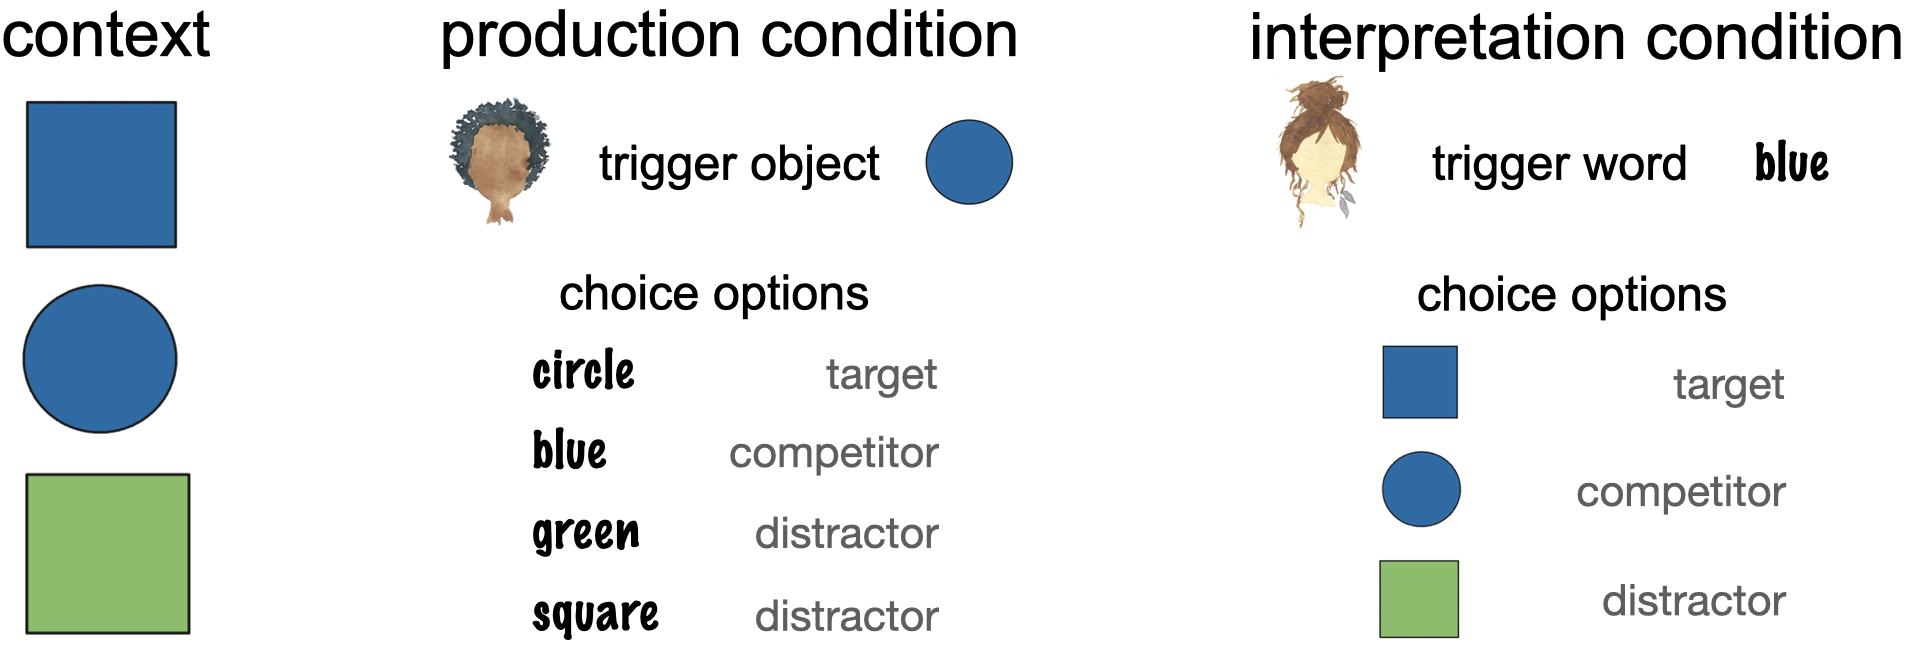
\includegraphics[width = 0.8\textwidth]{00-pics/reference-game.png}

  \caption{Structure of a reference game with human participants. Each trial consists of a set of objects, the so-called context. In production trials, participants choose a single word to describe a trigger object from the context. In interpretation trials, an object is selected as the likely object a trigger word referring to.}
  \label{fig:ref-game}
\end{figure}

Reference games are an established, well-understood and austere experimental paradigm to test human decision making in abstract communicative tasks \citep[e.g.,][]{FrankGoodman2012:Predicting-Prag,DegenFranke2013:Cost-Based-Prag,QingFranke2013:Variations-on-a,Frank2016:Rational-speech,SikosVenhuizen2021:Reevaluating-pr}.
A reference game consists of two players, a speaker and an interpreter, who jointly observe a set of objects, usually referred to as context (see Figure~\ref{fig:ref-game}).
In the \textbf{production condition}, the speaker is assigned a \emph{trigger object} from the context set which they have to describe to the interpreter.
In the \textbf{interpretation condition}, the interpreter observes a description, here called \emph{trigger word}, and chooses one of the objects from the context set.
The goal of the game is, for the speaker, to choose a description that enables the interpreter to choose the trigger object; and, for the interpreter, to guess correctly which object the speaker had in mind when using the trigger word.

The example in Figure~\ref{fig:ref-game} is a standard case, which we will use throughout, where human choices are informative about the pragmatic reasoning that human decision makers engage in.
In this example, there are two features that differ across three objects (here shape and color).
One object shares both its color and shape with one other object, while the two other objects have one unique feature (e.g., being the only circle, or the only green object).
%
In a critical production trial, the trigger object to describe is one of the two objects with a unique feature.
The speaker has four words to choose from.
The \textbf{target utterance} is the word which uniquely describes the trigger object.
The \textbf{distractor utterance} is the word that is true of the trigger object, but also true of another object.
The other utterances, both of which are false of the trigger object are \textbf{competitor utterance}.
%
In a critical interpretation trial, the trigger word is one that is true of two of the three objects.
If participants engage in pragmatic thought, they might reason that \emph{if} the speaker had wanted to refer to one of the two objects of which the trigger word is true (blue square and blue circle in Figure~\ref{fig:ref-game}), the speaker could have used a more informative word for exactly one of those two objects (``circle''), so they are more likely to refer to the \textbf{target object} (the blue square in Figure~\ref{fig:ref-game}).
The \textbf{competitor object} is the other object of which the trigger word is true.
The \textbf{distractor object} is the object of which the trigger word is false.

We replicated a simple reference game with human participants in which each trial instantiated the structure of the example shown in Figure~\ref{fig:ref-game}.
While previous reference games with human participants used pictorial representations of objects, and sometimes even pictorial representations of messages, we implemented a text-only version in order to be able to compare the predictions of LLMs for human data, when both LLMs and humans processed the same textual representation of the stimuli.
The experiment was realized as an online task using \texttt{magpie} \citep{FrankeJi:magpie:-Minimal}.\footnote{
  The code for the experiment can be found at \href{https://github.com/magpie-ea/magpie3-text-refgame}{https://github.com/magpie-ea/magpie3-text-refgame}, and a live version of the experiment can be tested at \href{https://magpie-ea.github.io/magpie3-text-refgame/}{https://magpie-ea.github.io/magpie3-text-refgame/}.
}


\subsection{Participants}
\label{participants}

A total of 302 participants were recruited via Prolific for monetary
compensation (\textsterling0.45, corresponding to roughly \textsterling 15.40 per hour).
All participants self-identified as native speakers of English.

\subsection{Materials \& design}
\label{materials-design}

We created 100 different items as stimulus material via a stochastic process.
Each item is a different textual description of a reference game with the same logical structure as the example from Figure~\ref{fig:ref-game}.
For each item, the context consisted of three objects.
As in the original paper by \citet{FrankGoodman2012:Predicting-Prag}, objects are defined by a triple of properties, namely a color, a shape and a texture.
For each property, there were four possible values, e.g., blue, green, red, and orange for color.
The sampled items differed in terms of the properties of the objects in the context set, and in terms of the order in which the objects and expression alternatives were presented in the text.
Figures~\ref{fig:refgame-screenshot-production} and \ref{fig:refgame-screenshot-interpretation} from Appendix~\ref{sec:scre-from-online} show example screenshots from the experiment.

\subsection{Procedure}
\label{procedure}

For each participant the experiment sampled four different items.
Participants first played two of these in the production condition, then the other two in the interpretation condition.


\subsection{Results}\label{results}

The overall distribution of choices that correspond to the target, competitor, and distractor states is shown in Figure~\ref{fig:refgame-counts}.\footnote{
  The production condition actually has two distractor choices.
  Here and in the following, these are lumped together as a single category, also when modeling random errors in later models.
  This is a simplification but does not change anything of substance.}
It is interesting that the distractor options were chosen rather often.
We also see that the number of target choices is higher in the production condition than in the interpretation condition.
This is in line with previous experimental results on human reference games.
% \citep{QingFranke2013:Variations-on-a}.
For example, in previous forced-choice reference games with human participants with pictorial presentations of objects, \citet{QingFranke2013:Variations-on-a} observed the following proportions of target, competitor and distractor options: $\tuple{0.882, 0.118, 0}$ in the production and $\tuple{0.492, 0.506, 0.003}$ in the interpretation condition (for 288 observations in each condition).

\begin{figure}[t]
  \centering

    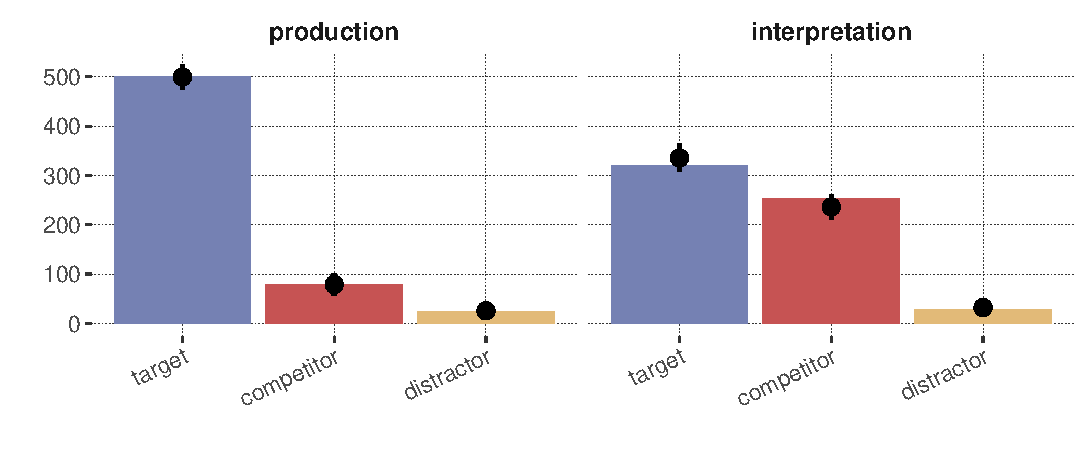
\includegraphics[width=0.9\linewidth]{00-pics/PPC-alpha-eps-model.pdf}

    \caption{Counts of choices from reference games with human participants (colored bars), with summary statistics from the posterior predictive distribution of four models (shapes and error bars).
      Shapes show the mean of the posterior predictive distributions of the RSA model and three further models derived from item-level LLM-supplied scores.
      Error-bars show corresponding 95\% credible intervals of the posterior predictive.
    }
  \label{fig:refgame-counts}
\end{figure}


%%%%%%%%%%%%%%%%%%%%%%%%%%%%%%%%%%%%%%%%%%%%%%%%%%
\section{Model predictions from probabilistic pragmatics}
\label{sec:model-pred-from}
%%%%%%%%%%%%%%%%%%%%%%%%%%%%%%%%%%%%%%%%%%%%%%%%%%

Data from reference games with human participants have been variously analyzed with probabilistic models using inspiration from behavioral game theory \citep[e.g.,][]{DegenFranke2013:Cost-Based-Prag}, probabilistic Bayesian modeling \citep[e.g.,][]{FrankGoodman2012:Predicting-Prag} or other forms of probabilistic modeling \citep[e.g.,][]{GattGompel2013:Are-we-Bayesian}.
Common to these approaches is that they derive or define, based on some explicit conceptual motivation, a parameterized stochastic speaker policy, $P_{S}(u \mid s; \theta_{S})$, modulated by parameters $\theta_{S}$, for a speaker's choice of expression or utterance $u$ given a referent or state $s$, which the speaker wants to communicate;
and a stochastic listener policy, $P_{L}(s \mid u; \theta_{L})$, capturing the probability of choosing a referent $s$ for utterance $u$.

As a concrete example, we introduce the Rational Speech Act (RSA) model first described in this form by \citet{FrankGoodman2012:Predicting-Prag} \citep[for overview see][]{FrankeJager2015:Probabilistic-p,GoodmanFrank2016:Pragmatic-Langu,StevensBenz2018:Game-Theoretic-,ScontrasTessler2021:A-practical-int,Degen2023:The-Rational-Sp}.
The RSA model defines pragmatic reasoning as a sequence of iterated (soft-)optmization of policies, grounding out in literal interpretation.
If $\mathfrak{L}(s,u) \mapsto \set{0,1}$ is a semantic meaning function mapping each pair of state $s$ and utterance $u$ to a (binary) truth-value, and if $P_{\text{prior}}(s)$ is a prior over states, a literal listener policy is defined as:
%
\begin{align*}
 P_{L_{0}}(s \mid u) \propto \mathfrak{L}(s,u)\  P_{\text{prior}}(s)\,.
\end{align*}
%
The pragmatic speaker policy is defined as soft-optimizing the choice of utterance to minimize the literal listener's surprisal for the state to be communicated, i.e., to maximize the log-probability of the trigger object:
%
\begin{align}
  \label{eq:RSA-speaker}
  P_{S}(u \mid s, \alpha) & \propto \expo \left [ \log P_{L_{0}}(s \mid u) \right ] \,.
\end{align}
%
Finally, the pragmatic listener is defined as the policy resulting from applying Bayes rule, solving the inverse-problem for the previously defined speaker policy:
%
\begin{align}
  \label{eq:RSA-interpreter}
  P_{L}(s \mid u, \alpha) \propto  P_{S}(u \mid s, \alpha) \  P_{\text{prior}}(s) \,.
\end{align}

\begin{figure}[t]
  \centering
  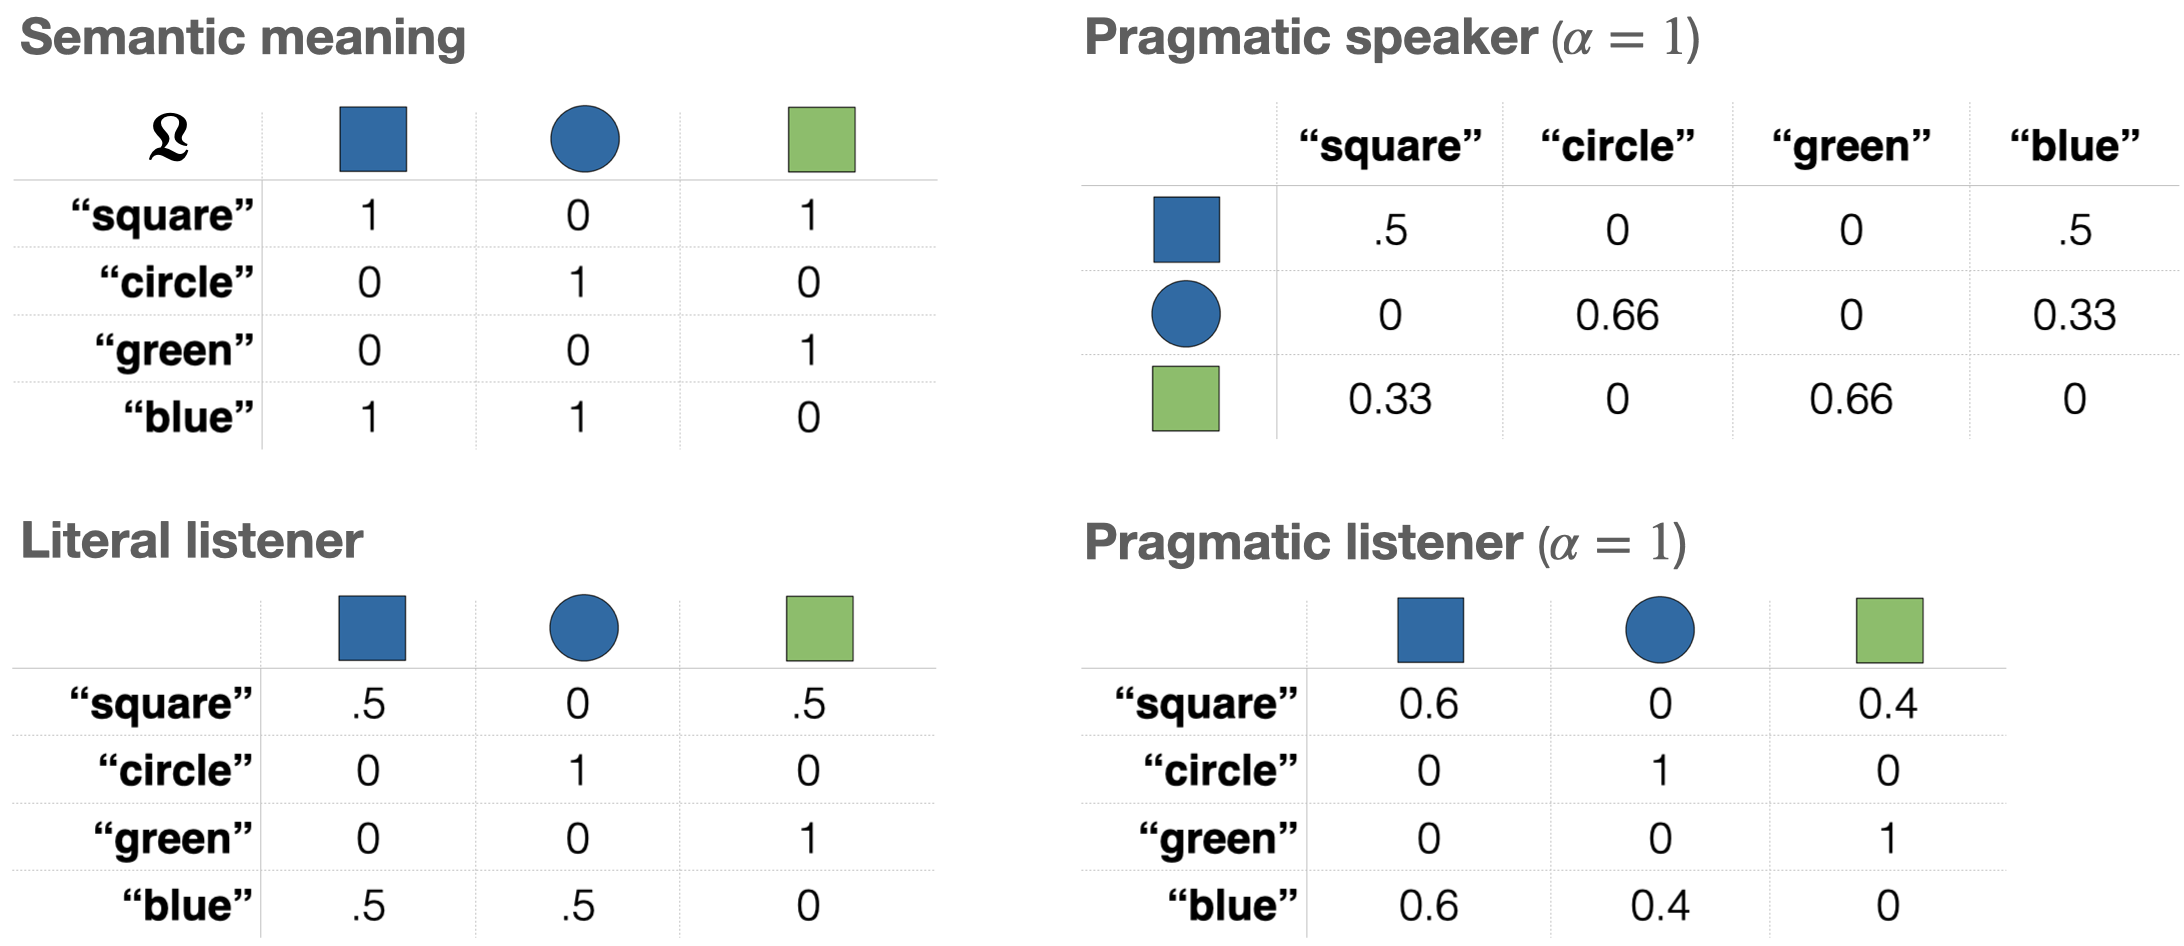
\includegraphics[width = 0.9 \textwidth]{00-pics/RSA-example.png}
  \caption{
    Example of predictions from the RSA model (with $\alpha=1$).
    The semantic meaning is shown as a matrix of binary truth-values.
    The policies of literal listener, pragmatic speaker and listener are calculated for uniform priors over state (referents) for $\alpha=1$ are shown as row-stochastic matrices.
  }
  \label{fig:RSA-example}
\end{figure}

Figure~\ref{fig:RSA-example} gives example calculations (assuming a flat prior and $\alpha=1$) for the reference game from Figure~\ref{fig:ref-game}.
For $\alpha=1$, the model predicts that the probabilities of target, competitor and distractor options are $\tuple{\nicefrac{2}{3}, \nicefrac{1}{3}, 0}$ for the production, and $\tuple{\nicefrac{3}{5}, \nicefrac{2}{5}, 0}$ for the interpretation condition.
Increasing $\alpha$ will increase the odds of target over competitor choices.
In sum, the condition-level predictions of the RSA model are a parameterized function $P_{\text{cond}}^{\text{RSA}}(R_{l}, C; \alpha_{c})$, assigning a probability to each response category $R_{l}$ (target, competitor, or distractor) in each condition $C$ (production or interpretation).

The model constructed so far predicts probability zero for distractor choices, so that the human data shown in Figure~\ref{fig:refgame-counts}, where the distractor option was chosen in both conditions, would immediately rule out the model entirely.
It is therefore common to include a small error probability $\epsilon$, with which a choice would be made at random \citep[e.g.,][]{LeeWagenmakers2013:Bayesian-Cognit}, so that we get:
%
\begin{align*}
  P_{r}(R_{l}, C; \alpha_{c}, \epsilon_{c}) = (1 - \epsilon_{c}) \  P_{r}(R_{l}, C; \alpha_{c}) +  \nicefrac{\epsilon_{c}}{3}\,,
\end{align*}
%
where $\epsilon_{c}$ is a (condition-specific) parameter giving the probability that a choice was made by randomly guessing.\footnote{
  Since the RSA model predicts probability 0 for the distractor option, this model is, in principle, able to predict any probability distribution over the three choice categories that is compatible with the order: $P_{r}(R_{t}) \ge P_{r}(R_{c}) \ge P_{r}(R_{d})$.
  Intuitively, this is because with $\epsilon=0$, $P_{r}(R_{d}, C; \alpha_{c}) = 0$, so that there is an $\alpha$ for any ratio of predicted choice probabilities for target and competitor, as long as the target probability is no smaller than the competitor probability.
  The $\epsilon$-transformation is essentially a linear shift in the probability simplex towards the maximum entropy prediction, so that every prediction which obeys the ordering restriction above can be made for some pair of $\alpha$ and $\epsilon$.
  This prediction-triviality is met in two ways.
  For one, the Bayesian priors on model parameters soft-constrain the model, so that the \emph{ex ante} credible predictions do rule out many logically possible observations.
  For another, we break the triviality by assigning a non-zero probability to the prediction for the distractor option.
  The same triviality problem lurks for the \emph{average-WTA} model introduced in Section~\ref{llm-predictions-for-reference-games}, and the same solution is applied to it.
}

The data $D_{C}$ from condition $C$, see Figure~\ref{fig:refgame-counts}, consists of counts for each response category.
The parameterized likelihood function entailed by the RSA model for condition-level data $D_{C}$ is:
%
\begin{align}
  \label{eq:RSA-likelihood}
 P^{\text{RSA}}_{\text{cond}}(D_{C} \mid C, \alpha_{C}, \epsilon_{C}) = \text{Multinomial}(D_{C}, \tuple{P_{r}(R_{l}, C; \alpha_{c}, \epsilon_{c}}_{1 \le l \le 3})\,.
\end{align}
%
The result is a four-parameter model, one pair of parameters per condition.

Parameterized predictions, like in Equation~(\ref{eq:RSA-likelihood}), can be assessed in the light of the empirical data with the usual tools of Bayesian data analysis \citep[e.g.][]{GelmanCarlin2014:Bayesian-Data-A,McElreath2016:Statistical-Ret,Lambert2018:A-Students-Guid}.
Let $\alpha_{c}\sim \text{log-Normal}(1,1)$ have a reasonably wide log-Normal prior, and let $\epsilon_{c} \sim \text{Beta}(1,15)$ have a Beta prior favoring small values.
Using Stan \citep{Team2023:The-Stan-Core-L} for Bayesian inference, we obtain estimates of posterior credible values of model parameters (summary statistics of which are shown in Table~\ref{tab:sumStats}).\footnote{
  Posterior samples where generated for four chains with 2000 samples each, after a warm-up of 1000 samples. The ``adapt-delta'' value was set to 0.99. Converge was checked with $\hat{R}$-statistics \citep{GelmanRubin1992:Inference-from-}.
}

\begin{table}[t]
\centering
\begin{tabular}{llllcrlcrcl}
  \toprule
  &&&& $\alpha$ &&& $\epsilon$ & \\ \cmidrule(r){4-6} \cmidrule(l){7-9}
  data & model & condition & $|$95\%\ & mean\ & 95\%$|$\ & $|$95\%\ & mean\ & 95\%$|$\ & Bpppv & \\
  \midrule

  item-level  & RSA                & production     & 2.62 & 3.13 & 3.69 & 0.08 & 0.12 & 0.16 & 0.29 &  \\
  item-level  & RSA                & interpretation & 0.21 & 0.67 & 1.08 & 0.08 & 0.14 & 0.19 & 0.21 &  \\
  item-level  & LLM                & production     & 0.15 & 0.19 & 0.24 & 0.00 & 0.07 & 0.16 & 0.00 & * \\
  item-level  & LLM                & interpretation & 0.08 & 0.11 & 0.14 & 0.00 & 0.09 & 0.22 & 0.00 & * \\
  cond.-level & RSA                & production     & 2.62 & 3.14 & 3.70 & 0.08 & 0.12 & 0.17 & 0.50 &  \\
  cond.-level & RSA                & interpretation & 0.27 & 0.68 & 1.13 & 0.09 & 0.14 & 0.19 & 0.51 &  \\
  cond.-level & avg. scores        & production     & 0.19 & 0.22 & 0.25 & 0.00 & 0.03 & 0.08 & 0.05 &  \\
  cond.-level & avg. scores        & interpretation & 0.15 & 0.18 & 0.20 & 0.00 & 0.02 & 0.05 & 0.00 & * \\
  cond.-level & avg. probabilities & production     & 0.86 & 1.03 & 1.22 & 0.08 & 0.12 & 0.17 & 0.47 &  \\
  cond.-level & avg. probabilities & interpretation & 0.36 & 0.46 & 0.59 & 0.00 & 0.04 & 0.10 & 0.00 & * \\
  cond.-level & avg. WTA           & production     & 0.86 & 1.04 & 1.22 & 0.08 & 0.12 & 0.17 & 0.48 &  \\
  cond.-level & avg. WTA           & interpretation & 0.15 & 0.37 & 0.58 & 0.03 & 0.12 & 0.18 & 0.49 &  \\

   \bottomrule \\
\end{tabular}
\caption{
  Summary statistics for model fits.
  Columns show the means and 95\% credible intervals for posterior samples for each parameter, as well as the Bayesian posterior predictive $p$-values for each model, condition and data level.
  Asterisks mark Bppp-values no higher than $0.05$, flagging relative inability to capture the structure of the data.
}
\label{tab:sumStats}
\end{table}

To assess goodness-of-fit, we use the \emph{posterior predictive distribution}, i.e., the model's predictions about data of the same size and structure as the training data.
Figure~\ref{fig:refgame-counts} shows summary statistics (means and 95\% credible intervals) for the posterior predictive distribution of the RSA model (among other models for condition-level data, which are to be introduced later).
We see that for both conditions the RSA model passes a ``visual posterior predictive check'' \citep{Kruschke2011:Doing-Bayesian-}, which require that the distribution of posterior predictions includes the observed choice rates for each answer option.
To corroborate the visual impression, Table~\ref{tab:sumStats} shows sample-based estimates of Bayesian posterior predictive $p$-values (Bppp values), using likelihood of the observed data as a test statistics.
These Bppp values approximate the probability that a model conditioned on observed data $D_{\text{obs}}$ predicts future data $D_{rep}$, of the same size and format as $D_{obs}$, that is at least as likely as the data $D_{\text{obs}}$ itself is (given the posterior predictive distribution).
Very small Bppp values indicate that the model might be inadequate for reproducing the data it was trained on, so to speak.
This is clearly not the case for the RSA model with Bppp values close to 0.5, as shown in Table~\ref{tab:sumStats}.
In sum, the condition-level predictions by the RSA model, a theoretically motivated PCM, are not discredited by the condition-level data.
Reversely, the RSA model seems to adequately capture the condition-level data.

We can also use the condition-level predictions for predicting the item-level data.
If the whole data set for condition $C$ is chunked into item-level data, $D_{C} = \tuple{D^{1}_{C}, \dots, D^{m}_{C} }$, the likelihood function for analysis at the item-level uses the same (condition-level) predictor to separately predict data from each item, so that the likelihood function becomes:
%
\begin{align*}
 P^{\text{RSA}}_{\text{item}}(D_{C} \mid C, \alpha_{C}, \epsilon_{C}) = \prod_{k = 1}^{m} \text{Multinomial} \left (D_{C}^{k}, \tuple{P_{r}(R_{l}, C; \alpha_{c}, \epsilon_{c}}_{1 \le l \le 3} \right )\,.
\end{align*}
%
Fitting the RSA model to the partitioned data set, we find estimates of Bppp values that do not discredit the model (see Table~\ref{tab:sumStats}).
This suggests that the item-level variation in the human data is not so pronounced as to provide strong evidence against the condition-level predictor from a theoretically motivated PCM.
In other words, the condition-level RSA predictions seem to adequately capture also the item-level data.


The following sections apply these tests of Bayesian model criticism also to models built around predictor values from LLMs.
Section~\ref{sec:item-level-pred} first looks at the item-level data, before Section~\ref{llm-predictions-for-reference-games} investigates different ways for deriving condition-level predictions.

%%%%%%%%%%%%%%%%%%%%%%%%%%%%%%%%%%%%%%%%%%%%%%%%%%
\section{Item-level predictions from LLMs}
\label{sec:item-level-pred}
%%%%%%%%%%%%%%%%%%%%%%%%%%%%%%%%%%%%%%%%%%%%%%%%%%

The RSA model's predictions are defined at the condition-level.
An LLM, on the other hand, first and foremost makes predictions about each item.
As mentioned previously, the items of the reference game experiment differ in which levels of features (color, shape, texture) instantiate the structure of the task shown in Figure \ref{fig:ref-game}, as well as the order of presentation of objects and words.
We expect both human and LLM predictions to vary between different items: e.g., humans seem to have preferences for some features \citep[e.g.,][]{QingFranke2013:Variations-on-a}, such as over-production of informationally irrelevant material \citep[e.g.,][]{DaviesKatsos2010:Over-informativ,Rubio-Fernandez2019:Overinformative,DegenHawkins2020:When-redundancy}; and machines may be susceptible to the presentation of the order of choice options. \mf{@PT references from the NLP literature on effects of prompt variation?}
It therefore becomes an empirical question of whether a standard item-level score from LLMs provides a good fit, if we aim at predicting the human data separately for each item, not as a condition-level average.

\begin{figure}[t]
  \centering
  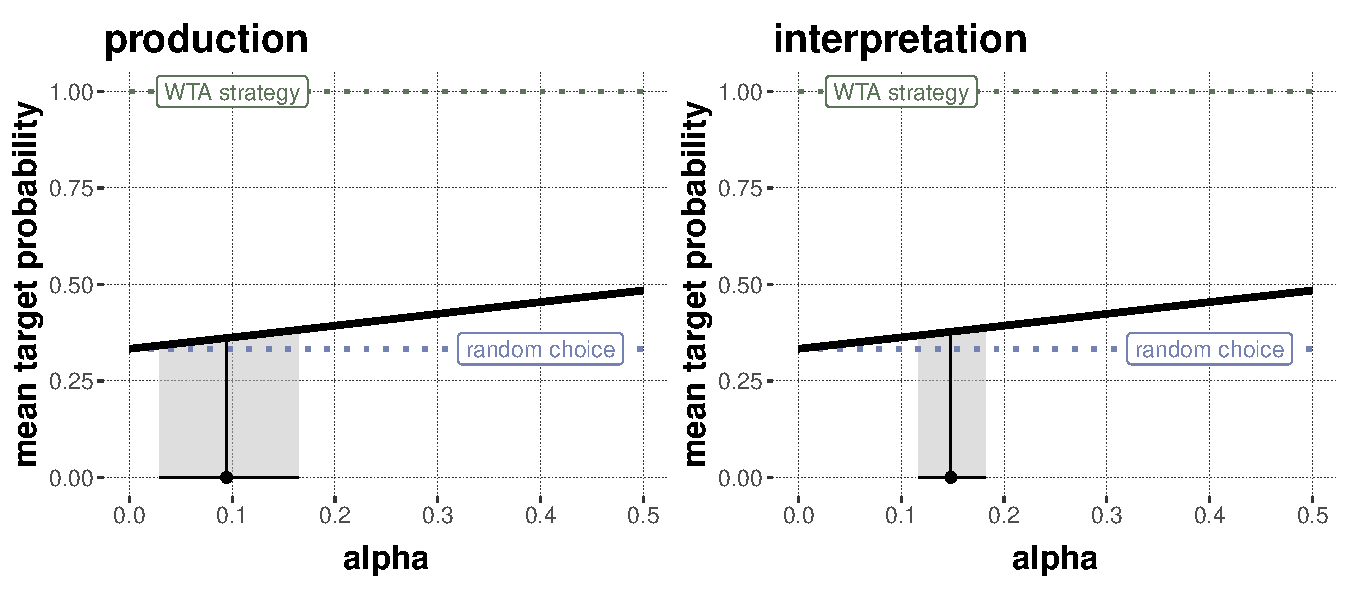
\includegraphics[width=\textwidth]{00-pics/closeness-target-by-alpha-item-level.pdf}
  \caption{
    Mean predicted target probability for different values of softmax parameter $\alpha$.
    The solid black lines show the probability of the target options, predicted for a fixed value of $\alpha$ ($x$-axis), averaged over all items for each condition.
    The gray-shaded area indicates the posterior 95\% credible interval for $\alpha$.
    For reference, the target probability under a random choice strategy and under the WTA strategy are shown with dashed lines.
    For credible values of $\alpha$, the means of predicted probabilities for the target option are clearly distinct from the WTA strategy.
  }
  \label{fig:closeness-target-item-level}
\end{figure}


As described in Section~\ref{motivation}, the standard procedure for assessing LLM predictions in multi-choice tasks is to use a winner-takes-all (WTA) strategy that just picks the best option for each item.
But since this strategy has conceptual and empirical weaknesses, we define the item-level LLM predictions using the more general softmax-approach, which contains the WTA-based approach as a limiting case, repeated here from above with slightly updated notation:
%
\begin{align*}
P_{\text{item}}^{\text{LLM}}\left ( y_{ki} \mid C; \alpha_{c} \right ) \propto \expo \left (\alpha_{c} \ \text{S}_{ki} \right)\,.
\end{align*}
%
Item-level scores $\text{S}_{ki}$, as defined in Section~\ref{motivation}, were obtained from the text-davinci-003 instance GPT-3.5 August 2023 \citep{BrownMann2020:Language-Models} .
% \footnote{
  % Numerically, we worked with \emph{average} log-probabilities. As in our experiment, all choice options had the same number of words, this is largely irrelevant, except for the effect of the $\alpha$ parameter in the interpretation condition. Using length-corrected log-probabilities is the same as using raw log-probabilities with an $\alpha$ parameter divided by the number of words. In this way, we make the $\alpha$ parameter more meaningfully comparable across conditions.}
The task description $x_{k}$ for item $I_{k}$ is a text supplied as prompt (see Appendix~\ref{sec:examples-items-llm} for an example).
The choice options are categorized as in the human experiment.\footnote{
  In the current set-up the response type ``distractor'' has two instantiations in the production condition. Since choice options are a single word in the production condition, for simplicity, we lump both of the distractor words together and treat them as a single option by taking the sum of the log-probabilities for both distractor words.}
Allowing for random errors with probability $\epsilon_{C}$, as before,:
%
\begin{align*}
  P_{\text{item}}^{\text{LLM}}\left ( y_{ki} \mid C; \alpha_{c}, \epsilon_{c} \right )
  = \epsilon_{c} \  P_{\text{item}}^{\text{LLM}}\left ( y_{ki} \mid C; \alpha_{c}, \epsilon_{c} \right ) \ \ + \ \ \nicefrac{\epsilon_{c}}{3}   \,.
\end{align*}
%
The resulting likelihood function for item-level data with item-level predictions is:
%
\begin{align*}
 P^{\text{LLM}}_{\text{item}}(D_{c} \mid C; \alpha_{c}, \epsilon_{c}) = \prod_{k = 1}^{m} \text{Multinomial} \left ( D_{c}^{k}, \tuple{P^{\text{LLM}}_{\text{item}}(y_{ki} \mid C;  \alpha_{c}, \epsilon_{c})}_{1 \le l \le 3} \right )\,.
\end{align*}
%
Priors on parameters are as for the RSA model described in Section~\ref{sec:model-pred-from}.

Summary statistics for samples from the posterior distribution over parameters are shown in Table~\ref{tab:sumStats}.
Credible values of $\alpha$ parameters are comparatively low for the LLM-based model, suggesting that the predicted scores have rather large differences, which have to be compensated for by the softmax link-function to adequately fit the data.
Figure~\ref{fig:closeness-target-item-level} shows the mean predicted target probabilities for different parameter values of $\alpha$, highlighting that for posterior credible values, the predictions are clearly distinct from the predictions of a WTA strategy.
This suggests that the WTA strategy, which is the special limiting case for $\alpha \rightarrow \infty$, provides a substantially worse fit for item-level choices than those provided by less extreme values of $\alpha$.

\begin{figure}[t]
  \centering

  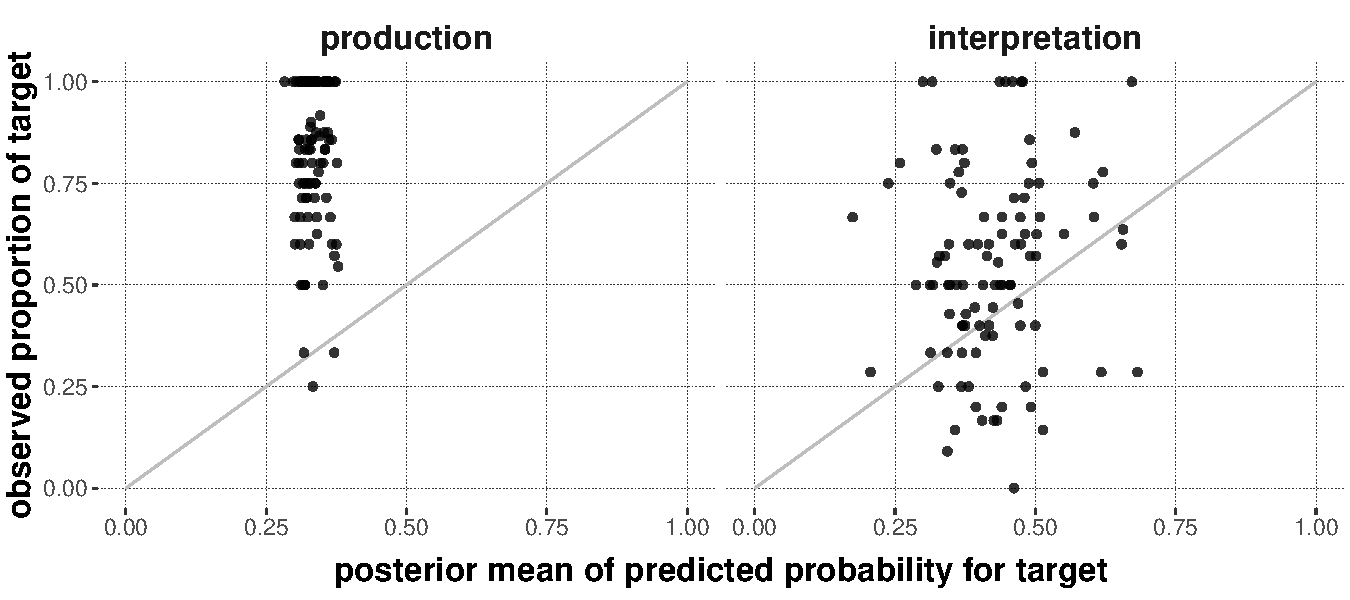
\includegraphics[width = 0.9\linewidth]{00-pics/item-combined-obs-pred.pdf}

  \caption{
    Item-level prediction-observation plot.
    Each dot represents an item.
    The $x$-coordinate represents the mean of the posterior prediction for the target choice probability for the given item.
    The $y$-coordinate represents the observed proportion of target choices for that item.
    The gray line (identity function) is the ideal prediction.
  }
  \label{fig:item-level-obs-pred}
\end{figure}

Sampling-based approximations of Bayesian posterior predictive $p$-values for the by-item analysis are very low (see Table~\ref{tab:sumStats}), suggesting that the unaggregated item-level LLM predictions are inadequate predictors of the human data.
Figure~\ref{fig:item-level-obs-pred} shows that the item-level LLM scores predict variance which is not borne out by the human data.
Concretely, the plots show, for each condition and item, mean posterior estimates of the model's predicted probability of choosing the target option ($x$-axis), together with the observed proportion of target choices in the human data ($y$-axis).
There is ample variation in the model's predictions, especially visible in the production condition, owing to the fact that the item-level scores of the LLM sometimes clearly favor another option than the target choice.
So, the model itself predicts systematic variability at the item level.
The human data, too, show variability at the item-level, but there is no (visual) indication that the item-level variability predicted by the LLMs is borne out by the human data.
These results suggest that LLM-based probabilistic predictions may imply item-level variance that is not attested in the human data.
Put more strongly, a model that uses the most obvious item-level score to predict what human participants choose on a by-item level is ruled out by experimental data.



%%%%%%%%%%%%%%%%%%%%%%%%%%%%%%%%%%%%%%%%%%%%%%%%%%
\section{Condition-level predictions}
\label{llm-predictions-for-reference-games}
%%%%%%%%%%%%%%%%%%%%%%%%%%%%%%%%%%%%%%%%%%%%%%%%%%

% This section explores different ways of deriving a probabilistic likelihood function for the human data from an LLM at the aggregate, condition-level.
% Using log-probabilities for each answer option as a basic item-level score, there are at least three conceivable ways of deriving condition-level predictions by averaging over item-level variation (see Figure~\ref{fig:measures-overview}).
% In the following, we first describe the different options of deriving LLM-based predictors.
% We then compare all probabilistic models based on their adequacy of explaining the human choice data.

\begin{figure}
  \centering
  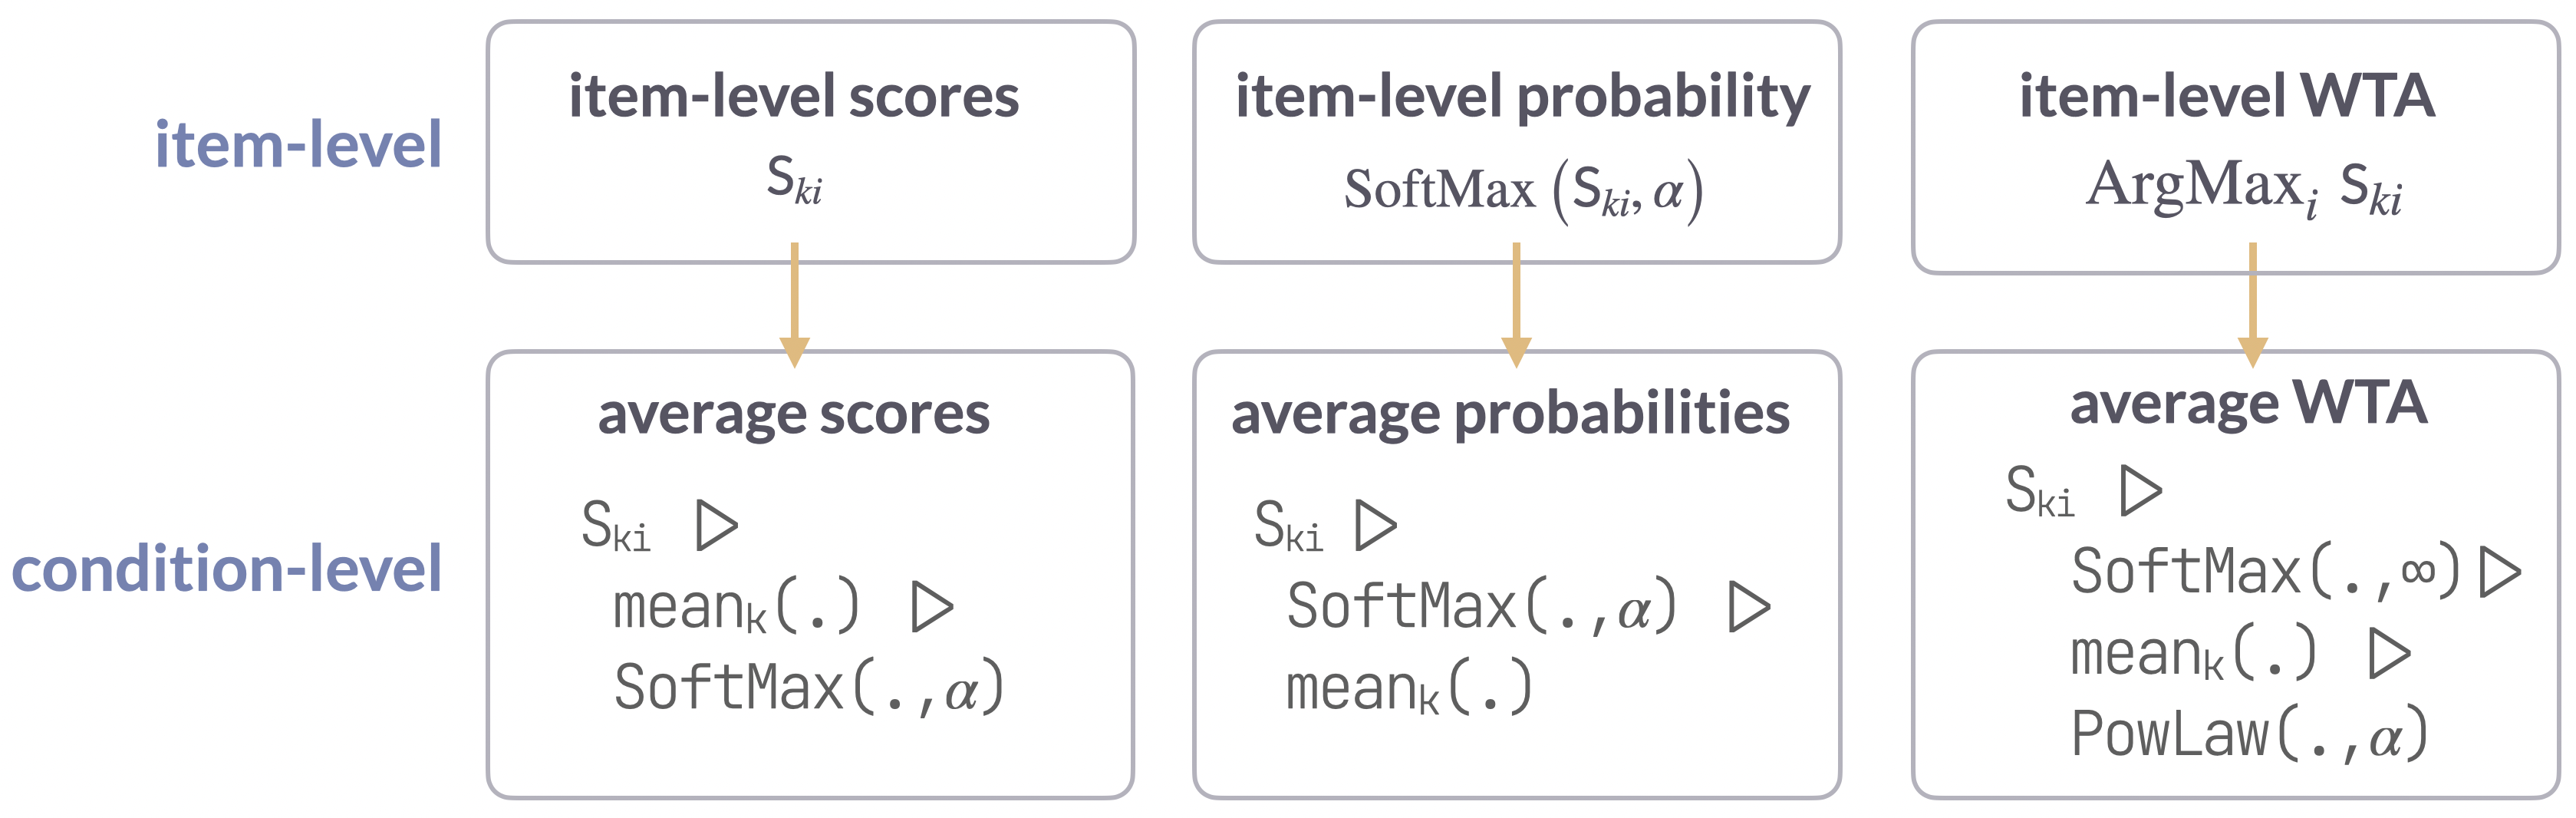
\includegraphics[width=0.9\textwidth]{00-pics/measures-overview.png}
  \caption{
    Schematic overview over three different approaches of obtaining condition-level predictions by aggregating item-level information.
    Approaches differ in the kind of item-level information they take into account, which entails differences in the order in which aggregation, transformation to probabilities and parameterized scaling occur.
  }
  \label{fig:measures-overview}
\end{figure}

While LLMs do not make conditional-level predictions as such, they can be derived from item-level scores $\text{S}_{ki}$ by averaging over all items belonging to the relevant condition.
There are many ways of averaging item-level information.
Figure~\ref{fig:measures-overview} shows three salient approaches, which differ in what the underlying item-level measure is: the raw scores $\text{S}_{ki}$, the item-level probability derived from it (as introduced in Section~\ref{motivation} and used in Section~\ref{sec:item-level-pred}), or the predictions from the winner-takes-all strategy commonly used in benchmark testing (see Section~\ref{motivation}).

% In general, to map a vector non-normalized scores $\myvec{s} = \tuple{s_{1}, \dots, s_{l}}$ to probabilities $\myvec{p} = \tuple{p_{1}, \dots, p_{l}}$ with different degrees of optimization, a common choice is the softmax function with optimality parameter $\alpha$:
% %
% \begin{align*}
%  \text{SoftMax}(\myvec{s}, \alpha) = \myvec{p}, \text{where } p_{i} \propto \expo \left (\alpha p_{i} \right )\,.
% \end{align*}
% %
% The softmax function can furthermore be decomposed into a first step of mapping scores to probabilities, and subsequently reweighing probabilities via a power-law transformation \citep[c.f.,][]{FrankeDegen2023:The-softmax-fun}:
% %
% \begin{align*}
%   \text{SoftMax}(\myvec{s}, \alpha) & = \text{Pow}( \text{SoftMax}(\myvec{s}, 1) ; \alpha) \\
%   \text{Pow}(\myvec{p} ; \alpha) & = \myvec{q}, \text{where } q_{i} \propto p_{i}^{\alpha}
% \end{align*}

The \emph{average-scores predictor} first aggregates the item-level scores, and then transposes the averages into (scaled) probabilities using the usual parameterized softmax function:\footnote{
  The reported results average over the multi-set \(\set{I_1, \dots I_m}\) of items that occurred in the human experiment for condition $C$.
  By using a multi-set, which may contain a single item multiple times, we produce aggregate predictions for exactly the set of items that the participant group saw, which provides the most fitting counterpart to the human data.}
%
\begin{align*}
  & P_{\text{cond}}^{\text{SCR}}(r_{i} \mid C, \alpha_{c})
    \propto \expo \left [  \alpha_{c} \ \frac{1}{m} \ \sum_{k=1}^{m} \text{S}_{ki}  \right ] \,.
    \tag*{\textcolor{gray}{[average scores (narrow-scope aggregation)]}}
\end{align*}
%
The \emph{average-probabilities predictor} first transposes scores into probabilities with a parameterized softmax function, and only aggregates over items last:
\begin{align*}
  % & \textbf{wide-scope aggregation} \\
  & P_{\text{cond}}^{\text{PRB}}(r_{i} \mid C, \alpha_{c})
    = \frac{1}{m} \ \sum_{k=1}^{m} P_{\text{item}}^{\text{LLM}}(y_{ki} \mid C, \alpha_{c}) \,.
    \tag*{\textcolor{gray}{[average probabilities (wide-scope aggregation)]}}
\end{align*}
%
Finally, the \emph{average-WTA predictor} considers the prediction of the WTA strategy as the basic item-level unit to aggregate over.
To add parameterized scaling to this method, a power-law transformation is a natural choice:
\begin{align*}
  % & \textbf{intermediate-scope aggregation} \\
  & P_{\text{cond}}^{\text{WTA}}(r_{i} \mid C, \alpha_{c})
    \propto  \left [ \frac{1}{m} \ \sum_{k=1}^{m} P_{\text{item}}^{\text{WTA}}(y_{ki} \mid C) \right ]^{\alpha_{c}}\,,
    \tag*{\textcolor{gray}{[average WTA (intermediate-scope aggregation)]}}
\end{align*}
where $P_{\text{item}}^{\text{WTA}}(y_{ki} \mid C) = \lim_{\alpha} P_{\text{item}}^{\text{LLM}}(y_{ki} \mid C, \alpha)$.
\bigskip


The \emph{average-scores} and \emph{average-probabilities} predictions are equivalent if there is only one item, in which case the prediction of the \emph{average-WTA} method is the special case of $\alpha \rightarrow \infty$.
For cases with more than one item, the predictions of the three predictors are not guaranteed to be the same.
Conceptually, the \emph{average-probabilities} and the \emph{average-WTA} predictors, but not the \emph{average-scores} predictor, are compatible with a picture in which condition-level predictions result from the actual predictions at the item level.
The difference between the \emph{average-probabilities} and the \emph{average-WTA} predictor is that the latter is an aggregate of an item-level predictor that is demonstrably bad, as shown in the previous Section~\ref{sec:item-level-pred}.

Using the same approach as for the RSA model in Section~\ref{sec:model-pred-from}, we can build likelihood functions for condition-level data around the three predictors introduced above.
With the same priors and methods used before, we obtain samples from the posterior over parameters and samples from the posterior predictive distributions.
Summary statistics for posteriors over model parameters are shown in Table~\ref{tab:sumStats}.
What is noteworthy is that for the \emph{average-WTA} model, the estimates of $\alpha_{c}$ in the production condition do not rule out, in fact lie close to, the special value $\alpha_{c}=1$, for which the power-law transformation is the identity function.
This means that just averaging WTA-responses at the item-level yields a reasonable predictor for the production data at the condition-level.
However, for the interpretation condition, the value $\alpha_{c}=1$ is clearly outside the range of credible parameter values, so that a simple recipe like ``always average WTA-responses without transformation'' is not a viable strategy for good condition-level predictions in general.
It is also worth noting that for the \emph{average-probability} model values of $\alpha_{c}$ close to one are virtually indistinguishable from the item-level predictions of the WTA strategy (see Figure~\ref{fig:closeness-target-item-level}).
This suggests that, for the production data, aggregation of item-level predictions from the WTA-strategy gives good condition-level predictions.
Since the production data is also very biased towards almost exclusively target choices by human participants, this is not too surprising.

Figure~\ref{fig:refgame-counts} shows the summary statistics (means and 95\% credible intervals) for each model's posterior predictive distribution.
We find that only the theoretical model (RSA) and the \emph{average-WTA} model pass this ``visual posterior predictive check'' for both conditions; the other two models both overpredict the target choice rate and underpredict the competitor choice rate in the interpretation condition.
To corroborate the visual impression, Table~\ref{tab:sumStats} shows sample-based estimates of Bayesian posterior predictive $p$-values, using likelihood of the observed data as a test statistics.
Consequently, the results from Table~\ref{tab:sumStats} suggest that the \emph{average-scores} model fails on the interpretation data, and is at most borderline compatible with the production data; that the \emph{average-probabilities} model is able to reproduce the production data, but fails on the interpretation data; and that only the \emph{average-WTA} model does not fail to capture the data from both conditions.

These results tell us that not all ways of deriving condition-level predictions by averaging over item-level variation are equally good.
Some approaches clearly fail basic checks for statistical goodness-of-fit.
On the positive side, we also find that there is at least one model with predictors based on LLM-measures, namely the \emph{average-WTA} model, which is able to recover the patterns in the data.
In other words, there is a way of deriving predictor values for condition-level forced-choice probabilities from an LLM such that, when fed into a common linking function (here with parameters $\alpha$ for optimization and $\epsilon$ for random error), the human choice probability can be reconstructed faithfully in its entirety.
On the other hand, there is a stark contrast between the results of item-level and condition-level data.
The model that was able to properly fit the condition-level data builds on predictions for item-level choice that are clearly incompatible with the human item-level data.
The model seems to be ``right for the wrong reasons.''



%%%%%%%%%%%%%%%%%%%%%%%%%%%%%%%%%%%%%%%%%%%%%%%%%%
\section{Conclusion}
\label{conclusion}
%%%%%%%%%%%%%%%%%%%%%%%%%%%%%%%%%%%%%%%%%%%%%%%%%%

While the common practice in evaluating the capabilities of LLMs is based on accuracy averaged over large collections of data, this work took the alternative route to explore what we learn if we subjected LLMs to the same routines and strong demands on distributional quality of fit to human data as we normally do for probabilistic cognitive models.
Taking this perspective, a main contribution of this paper is methodological, showing how statistical model criticism can be used for LLMs in the first place, and, more specifically, how it can be insightful in the detailed assessment of how LLMs might or might not be able to predict human data at the degree of accuracy that we would normally aspire for when dealing with explanatory statistical models in cognitive science.
Applying this comparative approach to a minimal, but non-trivial data set, we find that the LLM predictions on a per-item level predict variance that is not attested in the human data.
From several candidate predictor measures for aggregate condition-level data, only one was not refuted by the human data, but this was one that relied on the empirically implausible WTA-strategy at the item-level, incidentally the same strategy that is commonly used in accuracy-based benchmark testing \citep{srivastava2023-BIGbench}.

\paragraph{Explanatory power.}
The comparison of LLMs and PCMs led to a simple but consequential observation, namely that the atomic predictions or LLMs are at the item level, while explanatory PCMs usually make predictions at a more abstract level of conceptualization, similar to the level of an experimental condition.
This is one sense in which LLMs may be felt to be less, or not at all, explanatory.
They do not offer, at least not directly, a human-comprehensible compression of reality into a \emph{kind} of response pattern, over and beyond making a predicting for each particular situation.
As this kind of compression is arguably important for a sense of understanding \citep{Dellsen2020:Beyond-Explanat,Grimm2021:Understanding}, the direct comparison of LLMs with common practices in experimental psychology and with probabilistic cognitive models, provides an interesting perspective on why LLMs are often felt to be lacking in explanatory power.

This perspective on the explanatory role of LLMs goes beyond the factors of performance, indirect support and parsimony identified by \citet{SortNoopDeemtervan-Deemter2023:Dimensions-of-E}.
It is also subtly different from considerations of an LLMs ability to generalize \citep{HupkesDankers2020:Compositionalit}.
It rather suggests that \emph{transferability} is a dimension to ``explanatory power'' that is important as well.
Imagine that models $M$ and $M'$ have been designed for and trained on data from a situation $S$, but need to be applied to a different situation $T$.
Assume that for model $M$ the only way to make prediction for $T$ is to collect data pertaining to $T$, and either retrain or fine-tune the model.
In contrast, for model $M'$ can make predictions for $T$ without novel data collection by recognizing a meaningful difference between $S$ and $T$ and consequently manually changing parameter values or model-internal mechanics to accommodate for this change.
In that case, model $M'$ would be more transferable than model $M$.
For example, if we change the experimental setting for a reference game to consist of data from a special population, such as very young children or language-impaired adults, a potentially reasonable architectural change to a model like the RSA model is to consider differences in the sets of alternative utterances for the speaker \citep[e.g.][]{Noveck2001:When-Children-a}.
Even though this is only a vague explication of a notion of transferability, it suffices to corroborate the intuition that models like PCMs, which are designed to operate at a higher level of conceptual abstraction, will often appear more transferable than models like LLMs, which make predictions not for \emph{kinds} of situations but for \emph{particular} situations.
Whether any given model's transfer-ability is correct, is an orthogonal empirical question.
It is also an empirical question, exactly to which extent and in which areas LLMs are (not) transferable, especially if we consider prompting a transfer strategy \citep{LiuLiu2022:Generated-Knowl,XieRaghunathan2022:An-Explanation-}.
In any case, the comparison between LLMs and PCMs started here suggests systematic research into the transfer-ability and explanatory value of LLMs, e.g., by prompting strategies that are empirically insightful or by their use in composite neuro-symbolic models that implement theoretically-meaningful conceptual differences between types of situations.


\paragraph{Variability in predictions and performance measures.}
Despite being anchored in a small, but detailed case-study, the fact that different plausible methods of aggregating item-level information led to condition-level predictions of variable quality is worrisome.
Similarly, we argued that the wide-spread reliance on a winner-takes-all strategy might be inconsistent with the actual use practices of LLMs, which may not always rely on a temperature-zero sampling strategy (see Section~\ref{motivation}).
In conclusion, research on LLM should systematically study the conceptual and empirical consequences of seemingly minor decisions in evaluation or application settings.
Variability of performance measures also comes with a well-known risk for robust and reproducible science.
The more researcher degrees of freedom there are, the higher the risk of false results, even in the absence of intentions to mislead \citep[e.g.][]{Ioannidis2005:Why-Most-Publis,Chambers2017:The-Seven-Deadl}.
The comparison of LLMs with PCMs here raises awareness for the issue of robust research methods also in NLP \citep{WielingRawee2018:Reproducibility}.

The work presented here also contains considerable researcher degrees of freedom.
We only considered one out of several conceivable ways of carving a parameterized likelihood function from LLM-based predictors.
If future work would contribute to systematically exploring these, the main goal of this paper would have been met, which is to raise awareness for the possibility, perhaps even necessity, to scrutinize LLMs at the same level of rigorous detail as other models in cognitive science.

\paragraph{Human-like predictions from LLM.}
The question after the human-likeness of quantitative LLM-derived information matters for applications which use numerical scores to rank or weigh options \citep[e.g.,][]{ParkOBrien2023:Generative-Agen,ZhangLehman2023:OMNI:-Open-ende}.
Moreover, to the extent that LLMs are used as part of explanatory ``neuro-symbolic models'' of information processing \citep{GarcezLamb2020:Neurosymbolic-A}, understanding whether and how LLMs might yield full-fledged distributional predictions is important, e.g., to explore their integration into probabilistic (cognitive) models \citep[c.f.,][]{Frank2023:Large-language-}.
Based on the data set and the detailed analyses conducted here, it seems not infeasible to use numerical predictions from LLMs are part of predictive probabilistic models.
But, ideally, low-level variation, such as from order of presentation or similar ``nuisance variables,'' should be averaged out or taken into account in some way or other, at least as long as we do not understand what causes this variation in the predictions of models and further research that investigates when exactly this variation accords with empirically observed patterns.
In sum, we conjecture that using LLM predictors for probabilistic predictions, such as in a neuro-symbolic model, might be possible if embedded in the proper link functions and if item-level variation is taken into account.


\paragraph{No substitute for human subjects.}
Looking at LLM-derived predictions for human data from the perspective of cognitive modeling highlights the fact that LLMs predict item-level variation, but not subject-level variation, which is common in human data.
We may consider variation introduced via softmax / temperature as analogous to between-human variation, but this likely falls short of reality, where pronounced differences in answer behavior may surface.
For the particular case of pragmatic language use, prior research has shown that individual participants have markedly different behavioral profiles, often consistently behaving like literal language users or more sophisticated language users \citep[e.g.,][]{NieuwlandDitman2010:On-the-incremen,FrankeDegen2015:Reasoning-in-Re,SpychalskaKontinen2016:Investigating-s}.
It is an open question whether predictions from LLMs reflect the same kind of variation.
The results presented here recommend skepticism.
We therefore side with the cautious voices that do not recommend replacing human participants with LLMs in psychological research \citep{DillionTandon2023:Can-AI-language,HardingDAlessandro2023:AI-language-mod}.
In contrast, there is a challenge for LLM research.
The fact that aggregate predictions can track aggregate human behaviour means that the variance in on both sides is washed out to achieve a similar result.
This raises the issue of finding the systematic differences between LLMs and human answerers.
The task then would be to find cases where the differences do \emph{not} wash out and ask: What if anything do these cases share?

\paragraph{Limitations and follow-up work.}
The scope of our experimental investigation was deliberately small but perspicuous.
Focusing on the methodological contributions and details in performance assessments, we focused on a minimal non-trivial case study where we could triangulate LLMs, PCMs and human data.
This work may therefore serve as starting point for a wider investigation of more complex data sets and case studies in which LLMs are analyzed as and directly compared to explanatory PCMs.


\printbibliography[heading=bibintoc]

\newpage
\appendix


%%%%%%%%%%%%%%%%%%%%%%%%%%%%%%%%%%%%%%%%%%%%%%%%%%
\section{Screenshots from the online experiment with human participants}
\label{sec:scre-from-online}
%%%%%%%%%%%%%%%%%%%%%%%%%%%%%%%%%%%%%%%%%%%%%%%%%%

Figure~\ref{fig:refgame-screenshot-production} shows a trial from the production condition, Figure~\ref{fig:refgame-screenshot-interpretation} one for the interpretation condition of the online experiment.

\begin{figure}[H]
  \centering
  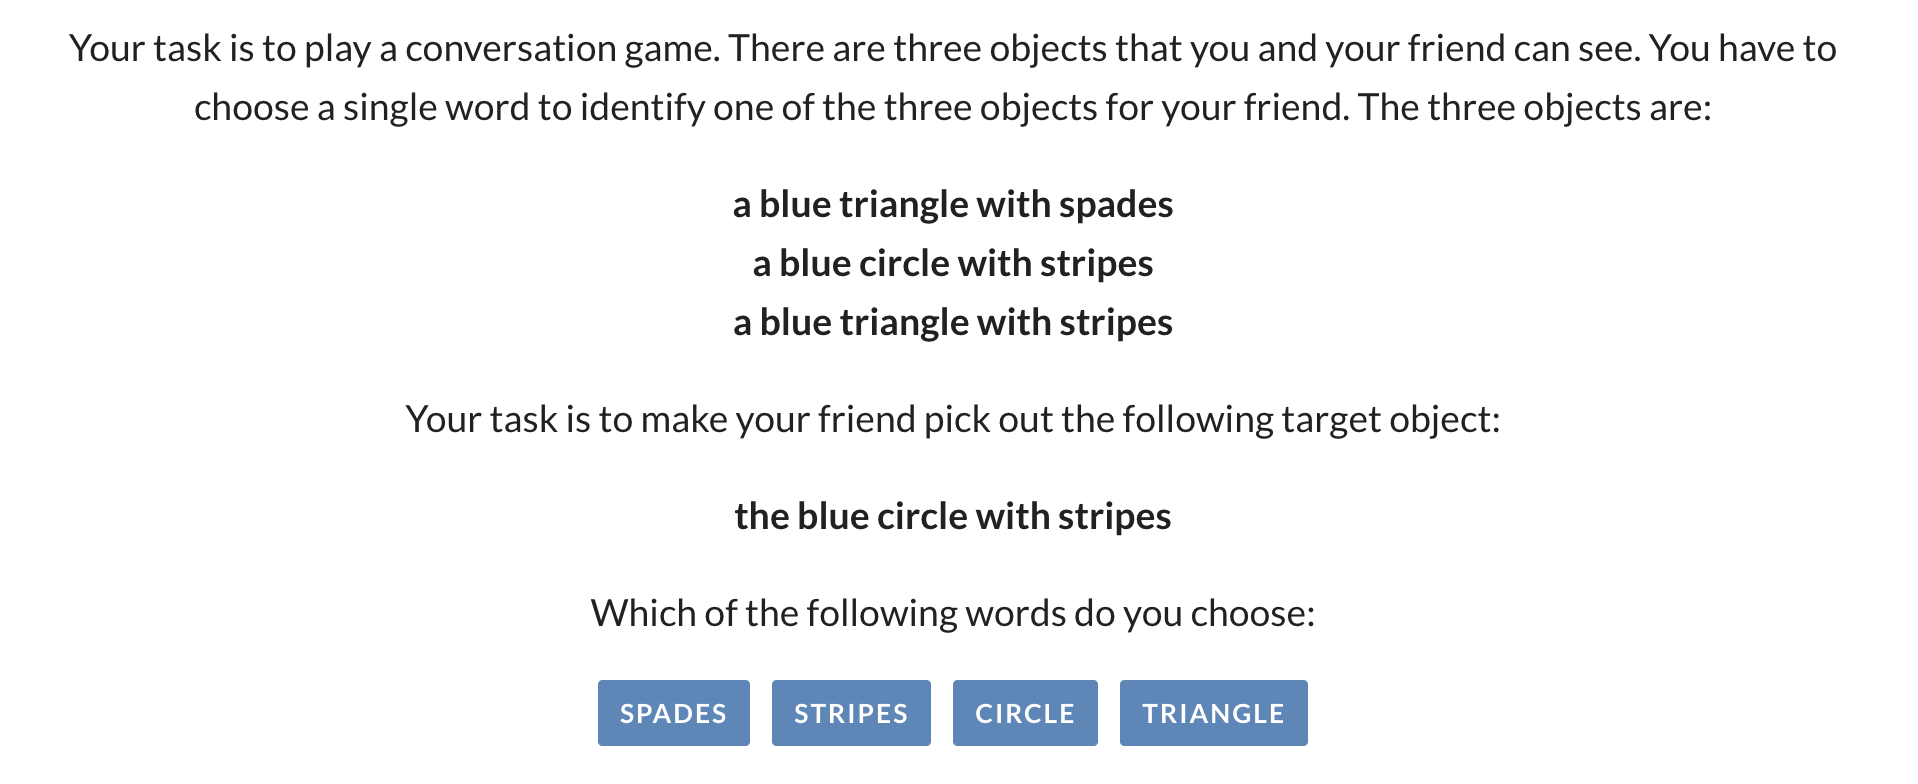
\includegraphics[width = 0.8\textwidth]{00-pics/refgame-production.png}

  \caption{Screen shot from a production trial of the online experiment.}
  \label{fig:refgame-screenshot-production}
\end{figure}

\begin{figure}[H]
  \centering
  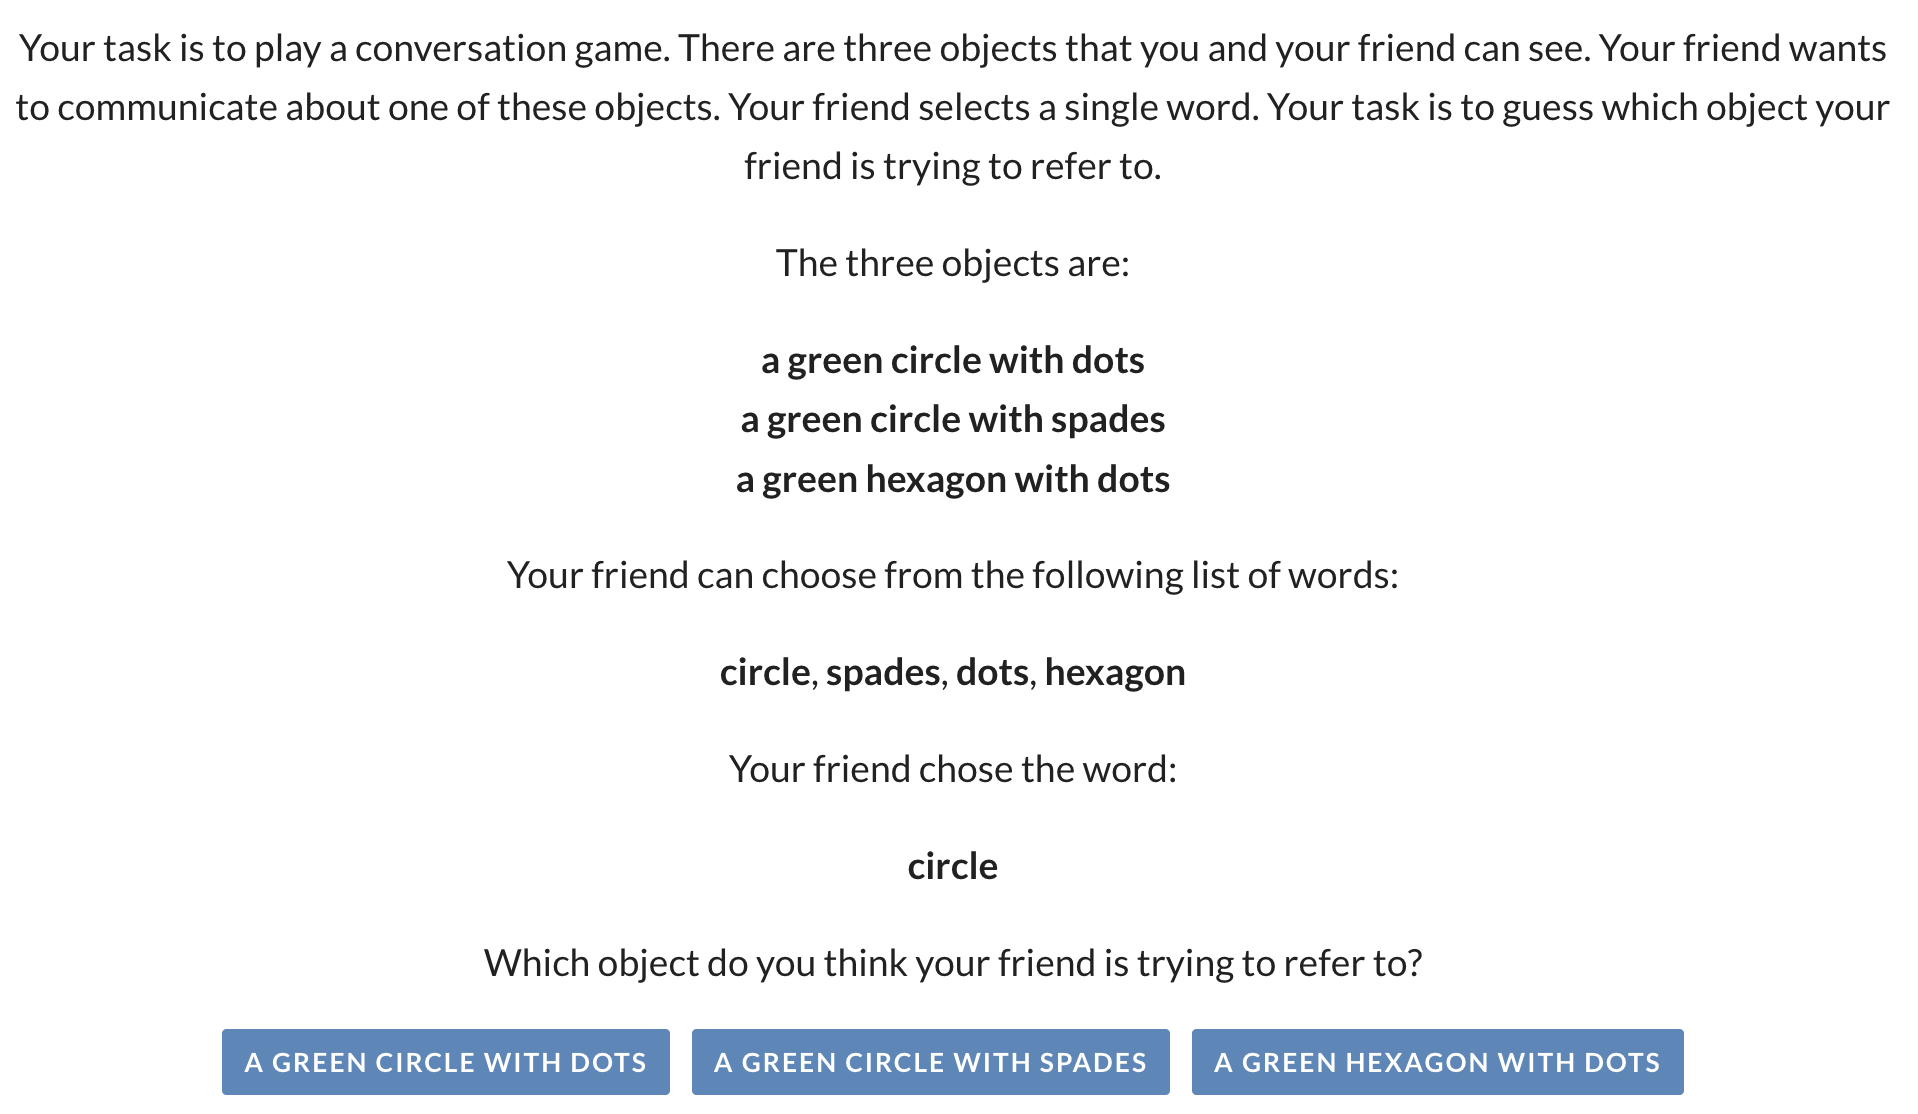
\includegraphics[width = 0.8\textwidth]{00-pics/refgame-interpretation.png}

  \caption{Screen shot from an interpretation trial of the online experiment.}
  \label{fig:refgame-screenshot-interpretation}
\end{figure}

\section{Example item for the LLM experiment}
\label{sec:examples-items-llm}

The text-based input for the LLM predictions mirrors the text in the human experiment, except that the LLM input also lists the set of all available choice options (which for the human experiment is unnecessary since this information is given by the buttons for the forced-choice selection).
For example, the task description $T_{k}$ for the item that corresponds to the production trial shown in Figure~\ref{fig:refgame-screenshot-production} is shown below (the actual input has no line breaks in the first paragraph):

\begin{verbatim}
Your task is to play a conversation game. There are three objects that
you and your friend can see. You have to choose a single word to identify
one of the three objects for your friend.

The three objects are:

a blue triangle with spades
a blue circle with stripes
a blue triangle with stripes

Your task is to make your friend pick out the following target object:

the blue circle with stripes

Which of the following words would you choose:

spades
stripes
circle
triangle

Your answer:

I would choose the word
\end{verbatim}


% %%%%%%%%%%%%%%%%%%%%%%%%%%%%%%%%%%%%%%%%%%%%%%%%%%
% \section{Range of prior predictions of intermediate-scope model}
% \label{sec:range-prior-pred}
% %%%%%%%%%%%%%%%%%%%%%%%%%%%%%%%%%%%%%%%%%%%%%%%%%%

% It may seem that, given the freedom to adjust optimization $\alpha$ and random guessing rate $\epsilon$, some models might be able to explain \emph{any} data observation.
% The intermediate-scope model, which was not discredited by model criticism in terms of recovery-based posterior predictive checks, is not trivial in this sense.
% Figure~\ref{fig:prediction-range} shows the range of predictions that the intermediate-scope model is, in principle, capable of making (for the whole possible range of \(\alpha\) and \(\epsilon\) values, disregarding Bayesian priors).
% There are distributions over response types which the model does not predict \emph{ex ante}.
% For example, the model does not predict cases where the number of competitor choices is almost as high as the number of target choice, as would be the case if participants would consistently \emph{not} engage in pragmatic reasoning.


% \begin{figure}[t]
%   \centering

%   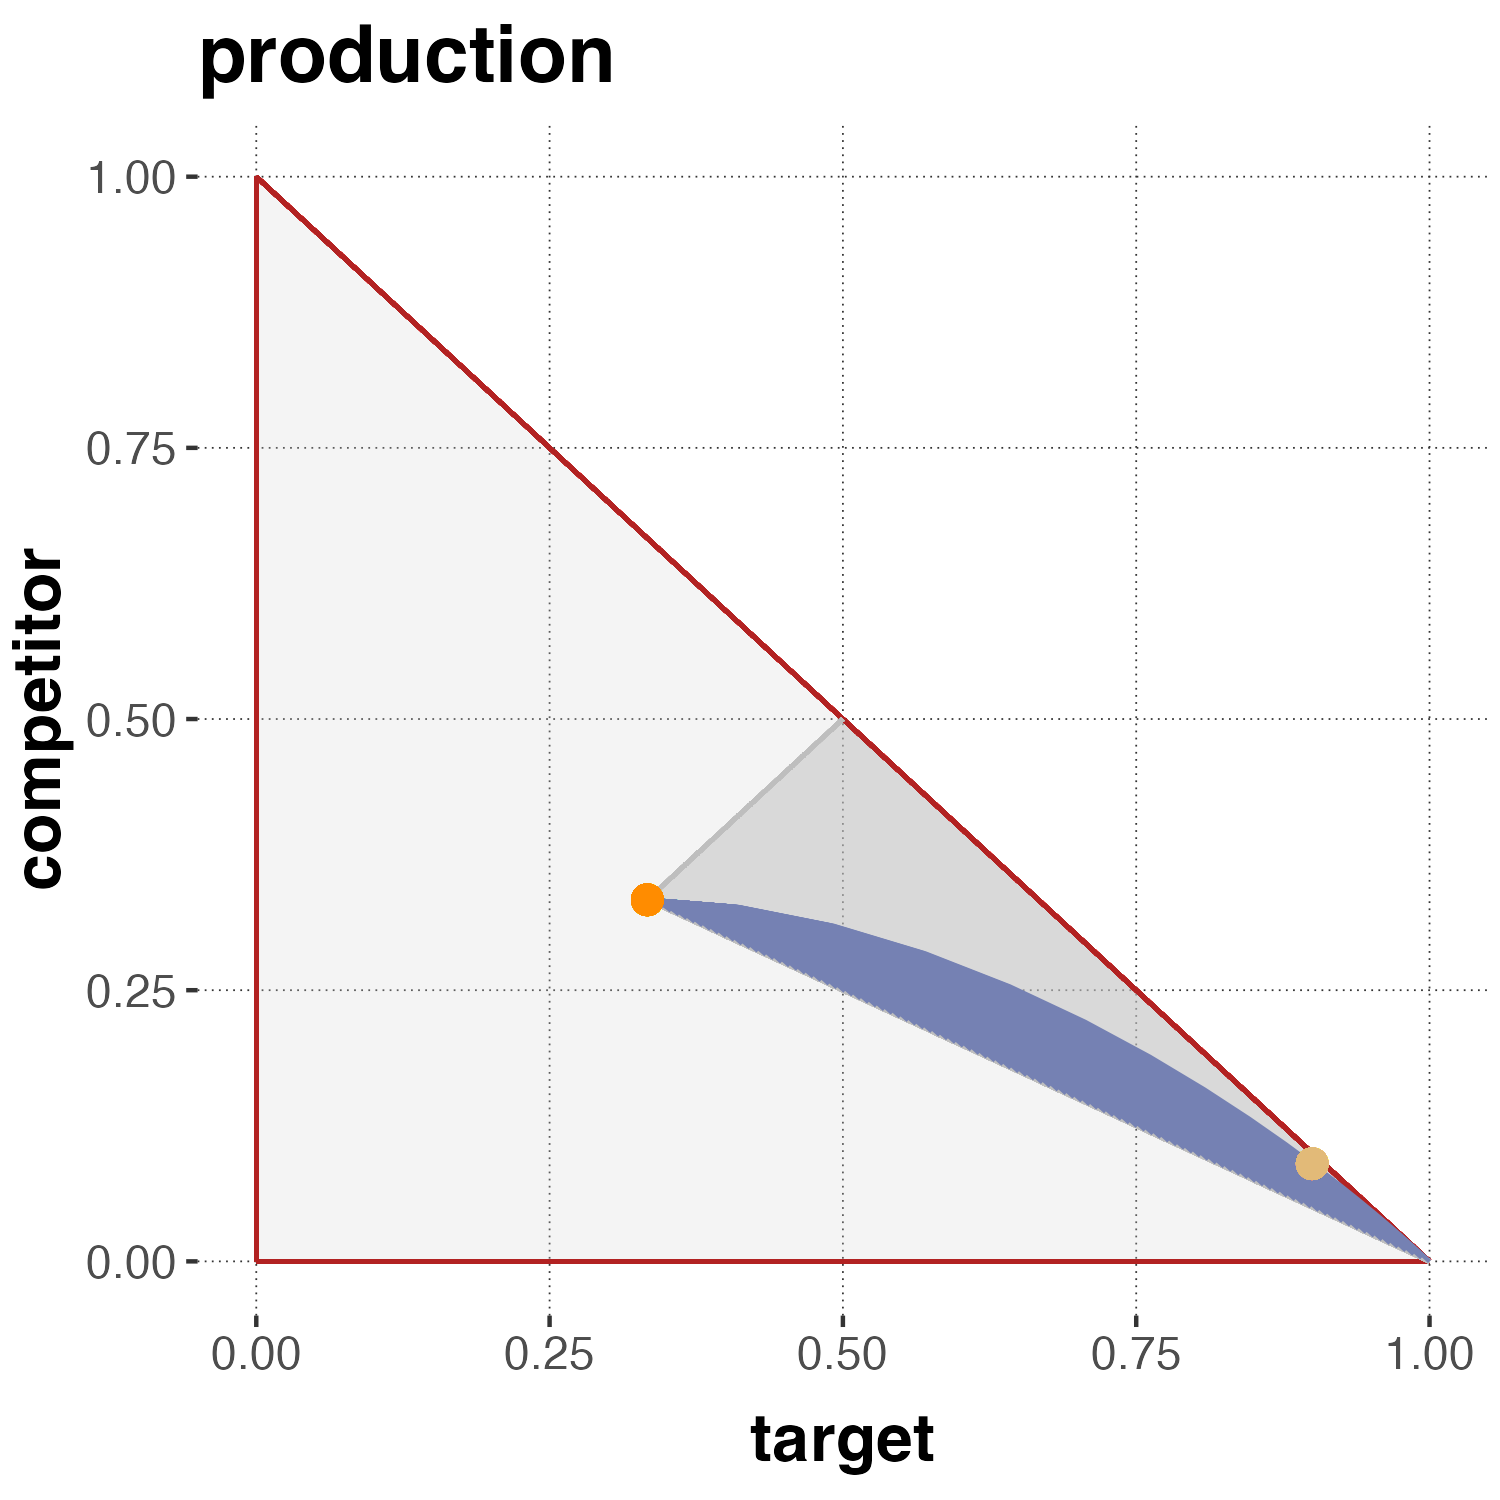
\includegraphics[width=0.45\textwidth]{00-pics/prediction-range-prod.png}
%   %
%   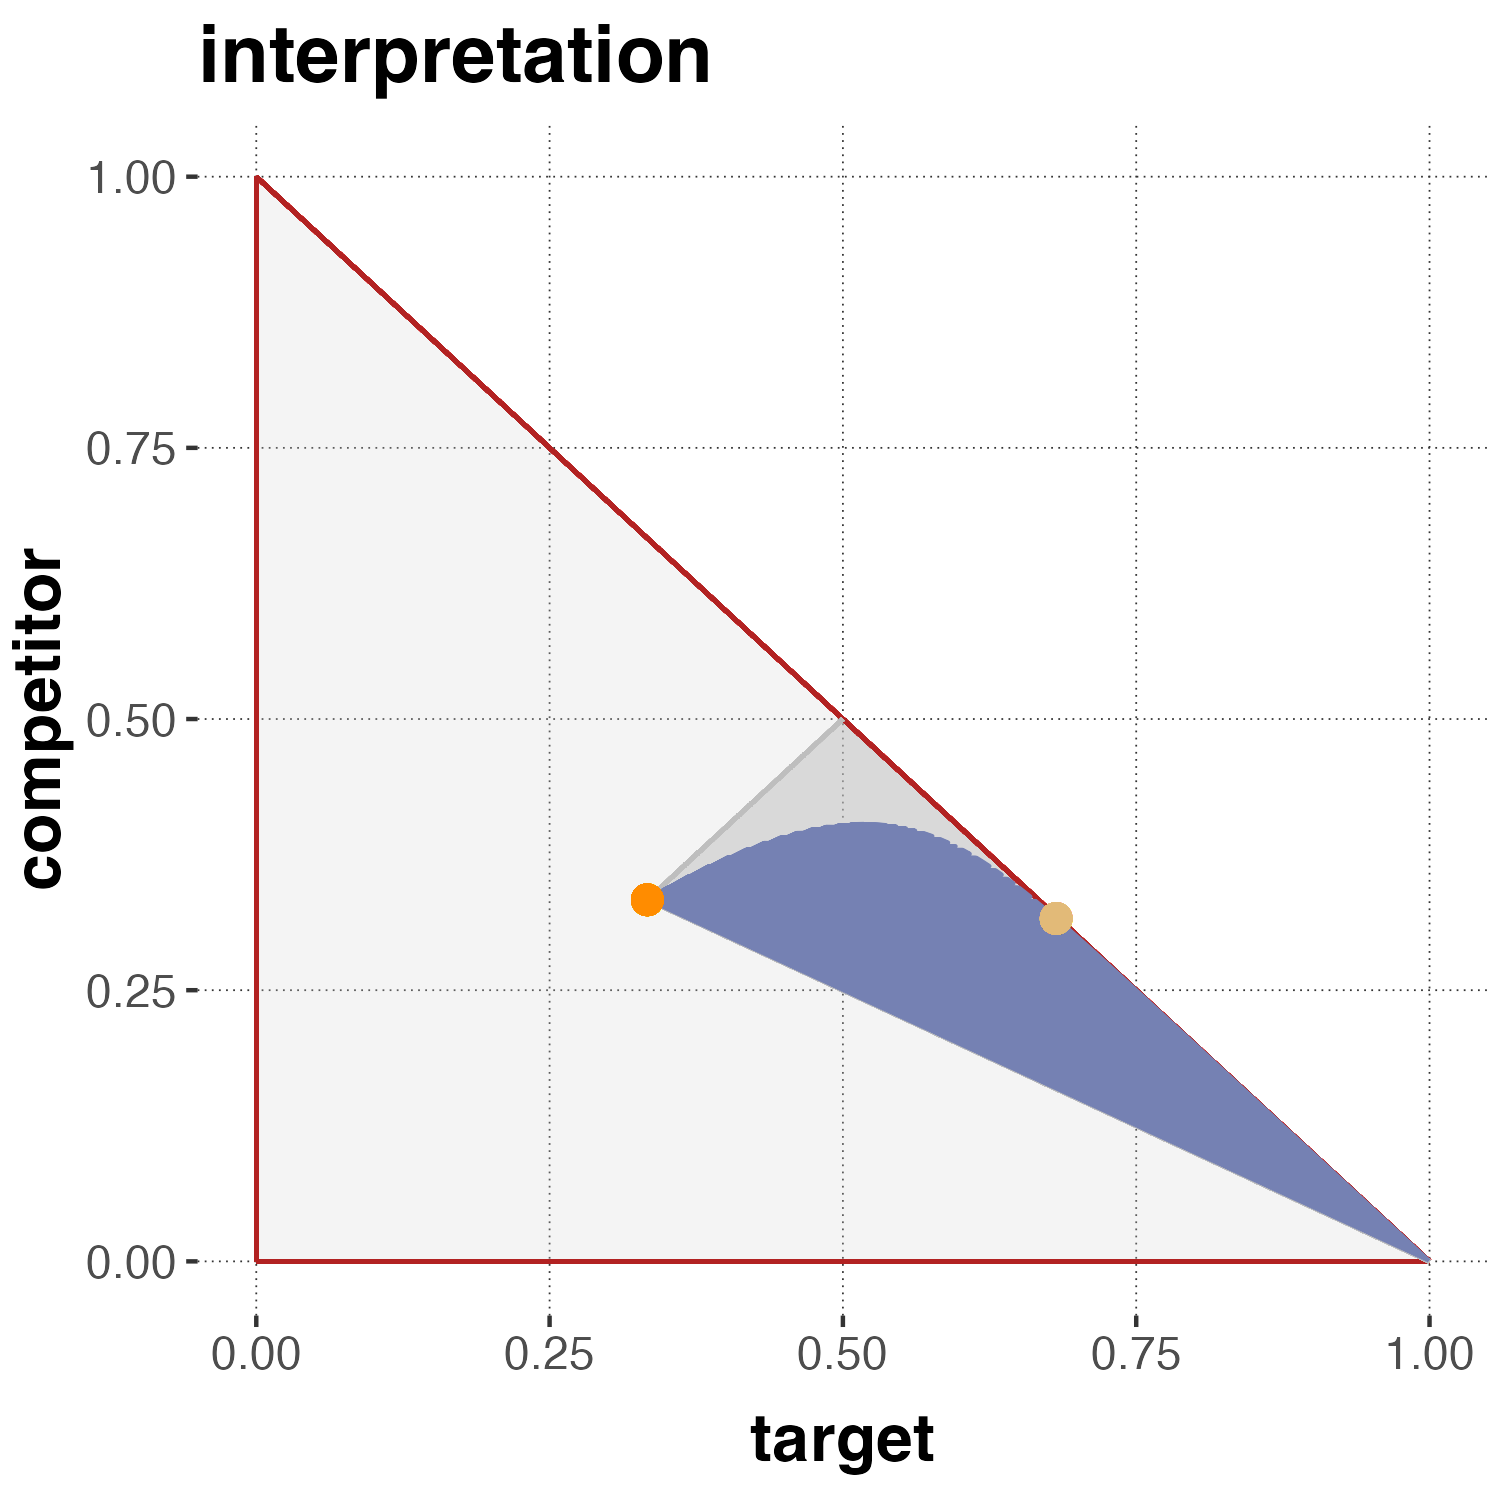
\includegraphics[width=0.45\textwidth]{00-pics/prediction-range-inter.png}

%   \caption{
%     Range of predictions the intermediate-scope model makes for any pair of parameter values $\alpha_{c}$ and $\epsilon_{c}$.
%     The light gray triangle with the red boundary is the probability simplex, i.e., the space of all possible 3-place probability vectors.
%     The darker gray area in gray boundary lines is the subspace that is compatible with the ordering that the probability of choosing the target is bigger than that of the competitor, which in turn is bigger than that of the distractor.
%     The blue area is the subspace of probabilistic predictions the intermediate-scope model makes under any value of its parameters.
%     The orange dot in the middle is the ``Laplace point'' of equal probability for all three options, which the model predicts for $\alpha=0$ or $\epsilon=1$.
%     The yellow dot is the ``vanilla prediction'' for $\alpha_{c}=1$ and $\epsilon_{c}=0$.
%   }
%   \label{fig:prediction-range}
% \end{figure}


\end{document}

%%% Local Variables:
%%% mode: latex
%%% TeX-master: t
%%% End:
